\documentclass[a4paper,twoside,12pt,chapterprefix=false]{scrbook}

\usepackage{amsmath,amssymb,amsthm}
\usepackage[footnotesize,sl,SL,hang,tight]{subfigure}  % helpful package for aligning figures next to each other
\usepackage{longtable} % tables over several pages
\usepackage[font={small,sl},hang,labelfont=bf]{caption} % configure captions
%\usepackage{captcont} % continue sufigures over several pages
\usepackage{booktabs} % publication quality tables for LaTeX
%\usepackage{showkeys} % shows the labels above the references for easier development

\ifpdfoutput{%
	\usepackage[pdftex]{graphicx}
	\usepackage[]{pdfpages} %for including full pdf pages
}{%
	\usepackage{graphicx}
}
\usepackage{rotating} % rotate figures

\usepackage{scrlayer-scrpage}
\KOMAoptions{headinclude}

% Font packages:
\usepackage{times}
\usepackage{helvet}   % sets sans serif font
\usepackage[T1]{fontenc}

%PDF hyperref config
\ifpdfoutput{%
	\usepackage[pdftex,
		bookmarks,
		bookmarksopen=true,
		bookmarksnumbered=true,
		pdfauthor={Luke Smith},
		pdftitle={Motion Priors for Pose Estimation and Animation Workflows},
		colorlinks,
		linkcolor=black,
		citecolor=black,
		filecolor=black,
		urlcolor=black,
		anchorcolor=black,
		menucolor=black,
		breaklinks=true,
		pageanchor=true,
		plainpages=false,
		pdfpagelabels=true]{hyperref}
}{}

\ifpdfoutput{%
	\pdfcompresslevel=9
	\pdfoutput=1
	\DeclareGraphicsExtensions{.pdf,.png}
}{}

\bibliographystyle{alpha}

% Uncomment the chapter / section you are working on.
%
%\includeonly{figures}
%\includeonly{tables}
%\includeonly{data-analysis}
%\includeonly{conclusion}
%\includeonly{appendix}

%\pagestyle{useheadings}

% A4
%
\topmargin -0.5in
\textheight 9.3in
\textwidth 6.3in
\oddsidemargin 0.18in
\evensidemargin -0.22in
\parskip 0.1in
\parindent 0in

\renewcommand{\arraystretch}{1.5}
\renewcommand{\baselinestretch}{1}

% commands
\newcommand{\Adjoint}{\mbox{\rm Adj}}
\newcommand{\Area}{\mbox{\rm Area}}
\newcommand{\ACos}{{\mbox{\rm Cos}^{-1}}}
\newcommand{\ASin}{{\mbox{\rm Sin}^{-1}}}
\newcommand{\ATan}{{\mbox{\rm atan2}}}
\newcommand{\Code}[1]{{\tt #1}}
\newcommand{\Complex}{\mbox{\bf C}}
\newcommand{\Cross}{{\mbox{\rm Cross}}}
\newcommand{\Mydddot}[1]{\mbox{\shortstack{$.$\hspace*{-1pt}$.$\hspace*{-1pt}$.$\\$#1$}}}
\newcommand{\Degree}{\mbox{\rm degree}}
\newcommand{\Diag}{\mbox{\rm Diag}}
\newcommand{\Dim}{\mbox{\rm dim}}
\newcommand{\Dist}{\mbox{\rm Distance}}
\newcommand{\IntTwo}{\int\!\!\int}
\newcommand{\IntThree}{\int\!\!\int\! \!\int}
\newcommand{\Kernel}{\mbox{\rm kernel}}
\newcommand{\Kross}{\mbox{\rm Kross}}
\newcommand{\Grad}{\nabla}
\newcommand{\Perp}{\mbox{\rm Perp}}
\newcommand{\Point}[1]{{\cal #1}}
\newcommand{\Rank}{\mbox{\rm rank}}
\newcommand{\Range}{\mbox{\rm range}}
\newcommand{\Real}{{\mbox{\rm I}\hspace*{-2pt}\mbox{\rm R}}}
\newcommand{\RealSbt}{{\mbox{\rm\scriptsize I}\hspace*{-2pt}\mbox{\rm\scriptsize R}}}
\newcommand{\Res}{\mbox{\rm resultant}}
\newcommand{\Sbt}[1]{{\mbox{\rm\scriptsize #1}}}
\newcommand{\MySign}{\mbox{\rm Sign}}
\newcommand{\SignSBT}{\mbox{\rm\scriptsize Sign}}
\newcommand{\Skew}{\mbox{\rm Skew}}
\newcommand{\Span}{\mbox{\rm Span}}
\newcommand{\SqrDist}{\mbox{\rm Distance$^2$}}
\newcommand{\Trace}{\mbox{\rm Trace}}
\newcommand{\TRN}{{\mbox{\rm\scriptsize T}}}
\newcommand{\Vector}[1]{\mbox{\bf #1}}
\newcommand{\VectorM}[1]{\mbox{\boldmath $#1$}}
\newcommand{\Volume}{\mbox{\rm Volume}}

\newcommand{\IVec}{\mbox{\boldmath $\imath$}}
\newcommand{\JVec}{\mbox{\boldmath $\jmath$}}
\newcommand{\KVec}{\mbox{\boldmath $k$}}
\newcommand{\LVec}{\mbox{\boldmath $\ell$}}
\newcommand{\RMat}{{\cal R}}
\newcommand{\QMat}{{\cal Q}}
\newcommand{\QCMat}{\overline{\cal Q}}

\newcommand{\Lerp}{\mbox{\rm lerp}}
\newcommand{\Slerp}{\mbox{\rm slerp}}
\newcommand{\Quad}{\mbox{\rm quad}}
\newcommand{\Squad}{\mbox{\rm squad}}

\newcommand{\subsubsubsection}[1]{{\sc #1}}

\newcommand{\ODer}[2]{\frac{d #1}{d #2}}
\newcommand{\ODerT}[2]{\frac{d^2 #1}{d {#2}^2}}
\newcommand{\ODerM}[3]{\frac{d #1}{d #2 \, d #3}}
\newcommand{\PDer}[2]{\frac{\partial #1}{\partial #2}}
\newcommand{\PDerT}[2]{\frac{\partial^2 #1}{\partial {#2}^2}}
\newcommand{\PDerM}[3]{\frac{\partial^2 #1}{\partial #2 \, \partial #3}}

% mass density symbol
\newcommand{\Den}{\delta}

% environments
\newenvironment{BArray}[1]{\left\{ \begin{array}{#1}}{\end{array} \right\}}
\newenvironment{Combin}{\left( \begin{array}{c}}{\end{array} \right)}
\newenvironment{Matrix}[1]{\left[ \begin{array}{#1}}{\end{array} \right]}

% "Figure" environment
\newtheorem{localFigure}{Figure}[chapter]
\newenvironment{Figure}[1]{
  \begin{center}
  \begin{minipage}{6in}
  \par\noindent\hspace*{0pt}\hrulefill
  
  \begin{localFigure} \label{#1}
}{
  \end{localFigure}
  \par\noindent\hspace*{0pt}\hrulefill
  \end{minipage}
  \end{center}
}

% "Table" environment
\newtheorem{localTable}{Table}[chapter]
\newenvironment{Table}[1]{
  \begin{center}
  \begin{minipage}{6in}
  
  \begin{localTable} \label{#1}
}{
  \end{localTable}
  \end{minipage}
  \end{center}
}

% "CDROM" environment for source code on disk
%\newenvironment{CDROM}[1]{
%  \label{#1} 
%    \includegraphics{cdrom.png} \hspace*{0.1in}{\tt PointShop3D}. \rm
%}{
%  $\bowtie$
%}

% TO DO search symbol
\newcommand{\TODO}{\mbox{\large\bf TO DO}}
\newcommand{\REFR}{\mbox{\large\bf REFR}}

%  Terminates current page and paragraph, makes sure next page starts on
%  an odd-number, and generates a completely blank page, without page markers,
%  if necessary.
\newcommand{\clearemptydoublepage}{\newpage{\pagestyle{empty}\cleardoublepage}}

%%% Shoemake's commands
\DeclareMathOperator{\prp}{\text{\scshape perp}}
\DeclareMathOperator{\rot}{rot}
\DeclareMathOperator{\N}{N}
\providecommand{\vmag}[1]{\lVert#1\rVert}
\providecommand{\mutate}[1]{\overleftarrow{#1}}
\providecommand{\T}[1]{{#1}^{\mathrm T}}
\newcommand{\cross}{\times}
\newcommand{\by}{\times}
\newcommand{\vect}[1]{\mathbf{#1}}
\newcommand{\mat}[1]{\mathbf{#1}} % or not
%\newcommand{\quat}[1]{\mathbf{#1}}
\newcommand{\quat}[1]{\ensuremath{\mathbf{\dot{#1}}}}
\newcommand{\vV}{\vect{v}}
\newcommand{\vU}{\vect{u}}
\newcommand{\vE}{\vect{e}}
\newcommand{\vUh}{\hat{\vect{u}}}
\newcommand{\mQ}{\mat{Q}}
\newcommand{\mR}{\mat{R}}
\newcommand{\mM}{\mat{M}}
\newcommand{\mA}{\mat{A}}
\newcommand{\mB}{\mat{B}}
\newcommand{\mI}{\mat{I}}
\newcommand{\mJ}{\mat{J}}
\newcommand{\mX}{\mat{X}}
\newcommand{\mY}{\mat{Y}}
\newcommand{\mZ}{\mat{Z}}
\newcommand{\qo}{\quat{1}}
\newcommand{\qi}{\quat{i}}
\newcommand{\qj}{\quat{j}}
\newcommand{\qk}{\quat{k}}
\newcommand{\xh}{{x}}
\newcommand{\yh}{{y}}
\newcommand{\zh}{{z}}
\newcommand{\ch}{c}
\newcommand{\sh}{s}
\newcommand{\gt}{\theta}


%%
%%
%%


\begin{document}

%% Define leading chapter pages
%
%\addtokomafont{chapter}{\setlength{\parskip}{190pt}}   % SEVERE HACK to keep spacing to chapter art work
\renewcommand*{\chapterheadstartvskip}{\vspace*{215pt}}  % different hack to keep spacing to chapter artwork
%\addtokomafont{chapter}{\rmfamily}        % remove this if you prefer sans-serif section titles
%\addtokomafont{section}{\rmfamily}        % remove this if you prefer sans-serif section titles
%\addtokomafont{subsection}{\rmfamily}     % remove this if you prefer sans-serif section titles
%\addtokomafont{subsubsection}{\rmfamily}  % remove this if you prefer sans-serif section titles
%\addtokomafont{paragraph}{\rmfamily}      % replace by \sffamily if you prefer sans-serif para titles
\addtokomafont{paragraph}{\sffamily}

\def\mychpstyleintl{%
{\noindent\setlength{\tabcolsep}{0pt}\setlength{\arrayrulewidth}{2pt}%
\begin{tabular}{c}
\\[100pt]
\begin{tabular}{lr}
\begin{tabular}{p{0.6\linewidth}}
\\
\end{tabular}
&
\begin{tabular}{p{0.4\linewidth}}
\rightline{{%
\sffamily%
\fontseries{bx}%
\fontshape{n}%
\fontsize{100}{120}%choose baselineskip to be 1.2 times font size
\selectfont
\thechapter}}
\end{tabular}
\end{tabular}\\[300pt]
\end{tabular}
}}

\newpagestyle{mychapterpagestyle}{{\protect\mychpstyleintl}{\protect\mychpstyleintl}}{}
\newpagestyle{myappendixpagestyle}{{\protect\mychpstyleintl}{\protect\mychpstyleintl}}{}
%%

%% macros e.g.
\newcommand{\mfytext}[0]{my fancy text}

%refs
\newcommand{\chpref}[1]{Chapter \ref{#1}}
\newcommand{\secref}[1]{Section \ref{#1}}
%\newcommand{\equref}[1]{Equation \ref{#1}} %better use builtin \eqref{}
\newcommand{\figref}[1]{Figure \ref{#1}}
\newcommand{\tabref}[1]{Table \ref{#1}}
\newcommand{\apxref}[1]{Appendix \ref{#1}}
%%

\hypersetup{pageanchor=false} % disabling anchors for title page to avoid warning

%% Replace this by your own design of a title page
%
%\title{Thesis Title}
%\author{My Name}
%\date{September 2042}
%\maketitle
%\clearemptydoublepage
% --- selfmade version ----
\begin{titlepage}
	\topmargin 1.0cm
	\oddsidemargin 0.0cm
	\evensidemargin 0.0cm
	%\textwidth 6.5in
	\centering
	\Huge
	\vspace{3.0cm}
	\textbf{\textsf{Motion Priors for Pose Estimation and Animation Workflows}} \\[2.0cm]
	%\includegraphics*[width=0.4\textwidth]{Figures/titlefigure} \\[4.0cm]
	\vspace{5.0cm}
	\sffamily
	\Large
	Luke Smith
	\\[0.8cm]
	\large
	Master Thesis
	\\
	April 2022
	\\[1.3cm]
	Prof. Dr. Robert W. Sumner
	\vfill
	\includegraphics*[width=0.3\textwidth]{Figures/ETH_logo} \hfill
	\includegraphics*[width=0.3\textwidth]{Figures/CGL_logo}
	\vspace{3.4cm}
\end{titlepage}
\clearemptydoublepage
%%

\hypersetup{pageanchor=true}
\pagenumbering{roman}
\setcounter{page}{1}

\chapter*{Abstract}

\TODO{Abstract}

\cleardoublepage
\chapter*{Zusammenfassung}

\TODO{translate to German}

%include task description here:
\cleardoublepage
%\includegraphics[viewport=3cm 0cm 20cm 27.5cm]{task_description} %better use includepdf below!
%\includepdf{task_description}
\cleardoublepage

%include acknowledgment here:
%\include{acknowledgment}

\tableofcontents
\cleardoublepage

\addcontentsline{toc}{chapter}{List of Figures}
\listoffigures
\cleardoublepage

\addcontentsline{toc}{chapter}{List of Tables}
\listoftables
\cleardoublepage

\pagenumbering{arabic}
\renewcommand*{\chapterpagestyle}{mychapterpagestyle}
\renewcommand*{\chapterformat}{} % show chapter titles only (no numbers)
% \setchapterpreamble[o]{...}  unfortunately does not move the \chapter output downwards


% ---- MAIN PART ----

% set counter to n-1:
\setcounter{chapter}{0}

\chapter{Introduction}

Introduction

- Existing pipeline description
    - 2d keypoints
    - 3d keypoints
    - Optimisation of cameras, ground plane, etc.
- Existing pipeline problems
    - Robustness
- Investigation: Motion Priors
    - Use for plausible motion

% set counter to n-1:
\setcounter{chapter}{1}

\chapter{Related Work}


This section describes references

\section{Pose Estimation}
The existing pipeline for 2D pose estimation is based on Open Pose \cite{openPose}.


\section{Motion Priors}

The authors of HuMoR \cite{humor} presented a novel approach for learning and using a plausible motion prior. They train a conditional VAE that learns a distribution over latent transitions, in a canonical reference frame, between $\textit{states}$ that consist of a root translation, 3D joint positions, joint angles, and the respective velocities. They most notably use this model as a prior in a 'test time optimisation', which generates plausible sequence motions optimising for an initial state and a sequence of transitions starting from frame by frame estimates (2D/3D joints or points clouds). This optimisation includes, alongside others, a motion prior term based upon the conditional distribution $p(z_t|x_{t-1})$ that encourages plausible motion for the learned sequence. Note that the CVAE decoder also predicts ground plan contact alongside change in state, which are used as regularisers during their main use case 'test time optimisation'. The test time optimisation can operate on many modalities, 2D/3D joints, point clouds, etc., as the optimisation contains a Data Term $\epsilon_{data}$ that can be tailored to the modality as the HuMoR state is information rich, containing 3D joints (hence can fit to 2D joints through projection or directly to 3D) and can parametrise the SMPL model (hence the SMPL mesh can be correlated to point clouds).

I would see the success of HuMoR in occlusion situations to be largly due to the SMPL prior.


HuMoR discussions:
\begin{itemize}
    \item They consider extending the method to include body shape parameters in the state an important direction for improved generalisation.
    \item They claim normalising flows and neural ODEs show potential but they only link to papers explaining these concepts and not actually using them for this purpose so not sure (Normalising flow: map to a simple distribution with an invertible function => tractable marginal likelihood (unlike with VAEs where we have to deal with an ELBO), but I'm not sure we care about the marginal likelihood in this case)
    \item They claim 'MVAE' does not work well
    \item The SMPL regularisation and the learned contional prior are important during training
    \item Assumptions:
    \begin{itemize}
        \item The method necessitates knowledge of the ground plane, which is presently needed (empirical observation) for convergence during training (as the dataset is of motions with a flat ground), and thus also at test time even though it is not conceptually necessary
        \item Assumes static camera
    \end{itemize}
    \item Limitations:
    \begin{itemize}
        \item Single person formulation
    \end{itemize}
\end{itemize}


The authors of HuMoR \cite{humor} were inspired by the Motion VAE \cite{TODO} paper. This paper uses an Conditional VAE (with assumed standard normal prior conditioning (vs. NN in HuMoR)) that directly outputs the next state (rather than the change in state in HuMoR). The model is used Autoregressively to predict motion (rather than the main presented use of HuMoR which is to fit motion to a sequence of existing 2D/3D joint predictions, though HuMoR can equally well be used autoregressively), and is trained with the typical ELBO in a supervised manner.
Some notes to self about MotionVAE
\begin{itemize}
    \item MotionVAE is used with Deep RL with the action space taken to be the latent space of the CVAE, with a reward function that defines goals of a character, the control policy walks through the actions space to guide the generative model in accordance with these goals. Could be interesting for interactive character animation
    \item Their state representation has some differences to HuMoR, notably that the root position his projected onto the ground.
    \item Contains a nice overview of motion prediction methods
    \item Latent dimension size: 32 (typical physics based humanoid degrees of freedom)
    \item Some notes about things they mention in the related work section:
    \begin{itemize}
        \item They cite [Wang et al. 2019] who train a stochastic generative model with output $\textit{processed by a refiner network to remove foot skating and add robustness}$.
    \end{itemize}
    \item Main differences to HuMoR
    \begin{itemize}
        \item c.f discussion section in HuMoR
        \item Conditional prior
        \item Predict change in motion
        \item Predict ground contacts
        \item Much additional regularisation in training
        \item Difference state representation
        \item Use of SMPL by HuMoR
        \item Difference in network architectures
        \begin{itemize}
            \item HuMoR just uses MLPs and MVAE decoder is a 'MANN-style mixture-of-expert neural network' (6 networks, gating network weighting their outputs)
            \item RELU in HuMoR, ELU in MVAE
            \item MVAE decoder has latent variable input at each layer (not sure about HuMoR)
        \end{itemize}
        \item 
    \end{itemize}
\end{itemize}


\subsection{Overview of Approaches}
We are most interested in models that learn plausible, task independent, human motion. These are refered to by \cite{MVAE} as $\textit{Motion-then-control}$ models. We limit our scope to parametric models.
\begin{itemize}
    \item MVAE \cite{humor}
    \begin{itemize}
        \item Standard normal CVAE
        \item Outputs next pose
        \item Decoder is mixture of networks
        \item Trained with rollout and scheduled sampling
        \item State positions referenced to root projection onto ground
        \item Nice investigation into using RL in the latent space for character control
    \end{itemize}
    \item HuMoR \cite{humor}
    \begin{itemize}
        \item Parametrised conditional prior CVAE
        \item Outputs change in state and person ground contacts
        \item SMPL regularisers (a subset of their state parametrises the SMPL model)
        \item Motion learned in a canonical reference frame (TODO: not sure about MVAE)
        \item Trained without rollout (I beleive?) 
        \item State positions referenced as in SMPL model (to $(0,0)$?)
    \end{itemize}

    \item $\textbf{TODO: Things I haven't looked into so deeply}$
    \item Mixture-density network RNNs (MDN-RNNS)
    \begin{itemize}
        \item Referenced in \cite{MVAE}
        \item Output a distribution as a gaussian mixture model
    \end{itemize}
    \item Time-convolutional autoencoders
    \begin{itemize}
        \item Referenced in \cite{MVAE}
        \item Learns a latent motion manifold
        \item Followup paper also referenced
    \end{itemize}
    \item Humor claims normalising flows and neural ODEs show potential but they only link to papers explaining these concepts and not actually using them for this purpose so not sure
\end{itemize}


\subsection{General notes}
Training VAEs:
\begin{itemize}
    \item Posterior collapse
    \begin{itemize}
        \item Decoder ignores latent variable and overfits to the training sequences
        \item MVAE: input latent variable at each stage of the decoder
        \item Weighting of $\beta$-VAE
    \end{itemize}
    \item Quality vs. generalisation
    \begin{itemize}
        \item Depends on weighting of KL and Reconstructions Losses
        \item MVAE find empirically that: $\textit{MVAE reconstruction and KL losses being within one order of magnitude of eachother is a good proxy to balance}$
    \end{itemize}
    \item Stable sequence prediction
    \begin{itemize}
        \item Not sure we care so much as we probably won't be extrapolating new sequences
        \item MAVE: Scheduled sampling during training - model progressively learns to deal with it's own predictions
    \end{itemize}
\end{itemize}
\chapter{Main}

\TODO{Intro to central work section}

A number of directions were explored during this thesis. To begin with, in \secref{sec:humor_investigation} and \ref{sec:humor_improvement}, an attempt was made at adapting a state of the art method, \cite{humor}. Next, a new approach to the problem alongside some novel architectures were explored to try and mitigate the issues encountered in \secref{sec:humor_improvement}.

\section{HuMoR Investigation}
\label{sec:humor_investigation}

\TODO{Describe the humor method better, update the hand drawn diagrams with draw.io, read through and check everything is correctly introduced and I'm not assuming any pre knowledge of Humor}

The authors of \cite{humor} propose a compelling approach to the problem of learning a human motion model (namely the HuMoR model), alongside a well described method for employing this model in the task of improving a sequence of independently estimated 2d poses obtained from video data (this method is referred to as 'TestOps').  Considering that our problem definition matched exaclty this TestOps, that our desire was to use a motion model with the intuition that it would improve motion prediction in certain important situations such during occlusion, and the promising results showed by the paper, it was deemed that HuMoR represented a sensible starting point for our research.


\TODO{Describe the HuMoR method in more detail}

\subsection{Method}
Our investigation began with a largely qualitative evaluation of the HuMoR model, which had two main aims.  First was to stress test the system, to see where it failed, where it succeded, and if the mentioned benefits in the HuMoR paper \cite{humor} were as described.  Second was to evaluate the model with the defects of the current Disney system in mind to see if it could complement it's functionality.
The current systems most notable failure points arise in occluded situations?? \TODO{Any other failure cases}

To acheive this goal, a selection of videos were taken in the lab containing a variety of motion; fast, slow, and abnormal, and a including number of occluded scenes.  The HuMoR system was ran on these videos and the results were investigated.  The TestOps is performed in 3 stages, where only the 3rd makes use of the HuMoR motion model, we could therefore compare the stage 2 results to the stage 3 results to see where the model was providing an improvement over a more classical optimisation that includes smoothness and pose prior losses.


\subsection{Advantages of HuMoR}
We see a number of situations in which the model shows a clear improvement over the stage where the HuMoR model is not used.

In an occluded situation, as shown in \figref{fig:humor_sitting}, where the 2d pose predictions don't have any information on the legs, the model manages to produce a realistic sitting motion.

\begin{figure}[h!]
    \centering
    \subfloat[OpenPose]{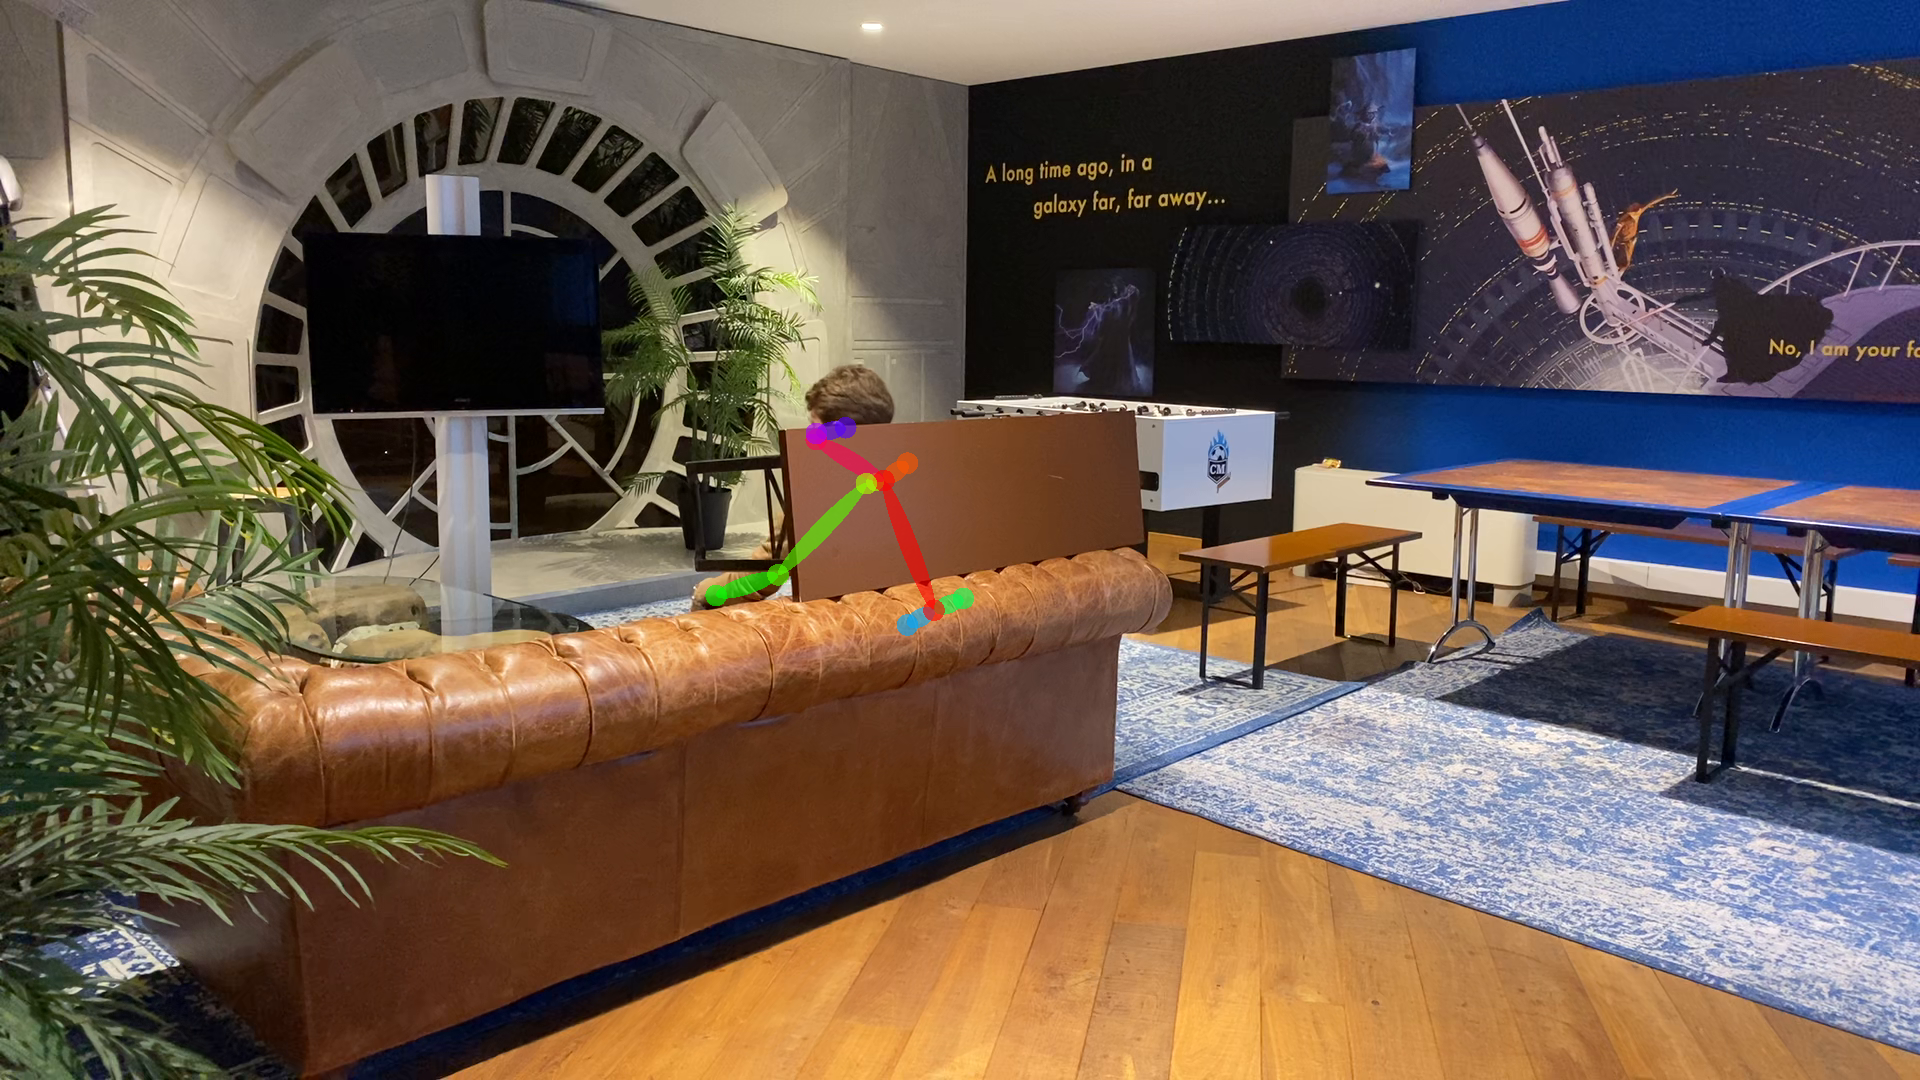
\includegraphics[width=0.3\textwidth]{Figures/humor/qualitative/good/sitting/openPose.png}} 
    \hfil
    \subfloat[Stage 2]{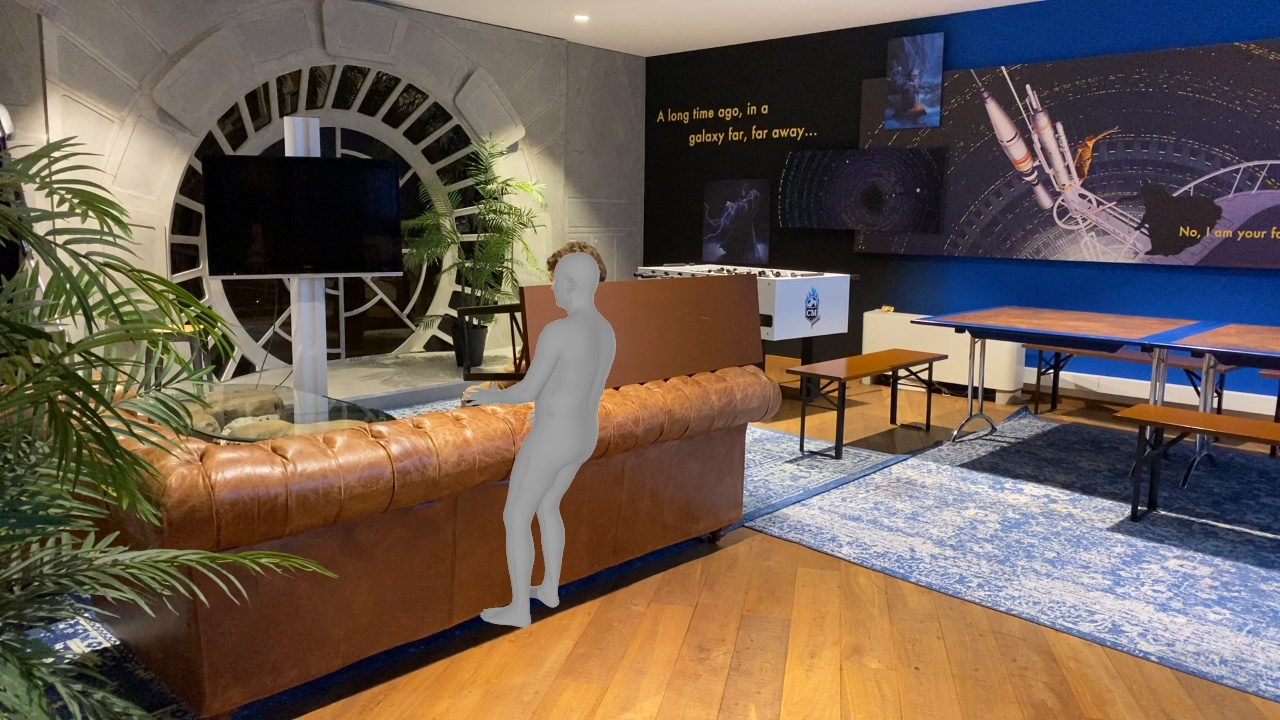
\includegraphics[width=0.3\textwidth]{Figures/humor/qualitative/good/sitting/stage2.jpg}} 
    \hfil
    \subfloat[Stage 3]{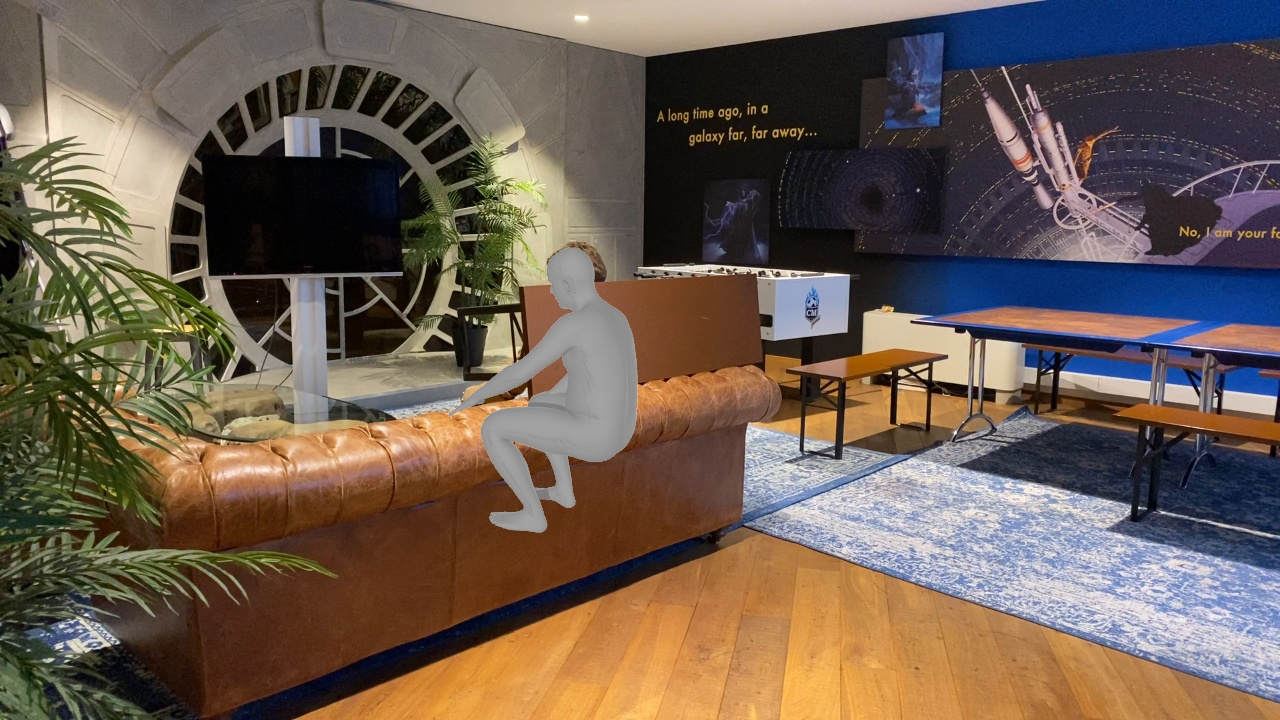
\includegraphics[width=0.3\textwidth]{Figures/humor/qualitative/good/sitting/stage3.jpg}}
    \caption{HuMoR achieving occluded sitting}
    \label{fig:humor_sitting}
\end{figure}

We also note in many of the less difficult videos, that HuMoR produces clean motion and deals with many abnormal movements without obvious issues. It therefore doesn't seem to regress the easy situations, but can improve the more difficult situations, notably occlusions.


\subsection{Drawbacks of HuMoR}

We noted that while HuMoR manages to sit when occluded, it often fails to walk. This seems to be due to the fact that OpenPose often predicts both legs on the frames just before the occlusions where only one leg is actually un-occluded, as can be seen in \figref{fig:humor_bad_occluded_walking}. This results in a sequence of poses where the frames before an occlusion indicate that the person is no longer walking, hence making it significantly more difficult for HuMoR to begin walking again during the occlusion. This issue is thus probably largely due to HuMoRs' TestOps' dependence on OpenPose and thus it's inheritence of OpenPoses' failure points.

\begin{figure}[h!]
    \centering
    \subfloat[OpenPose]{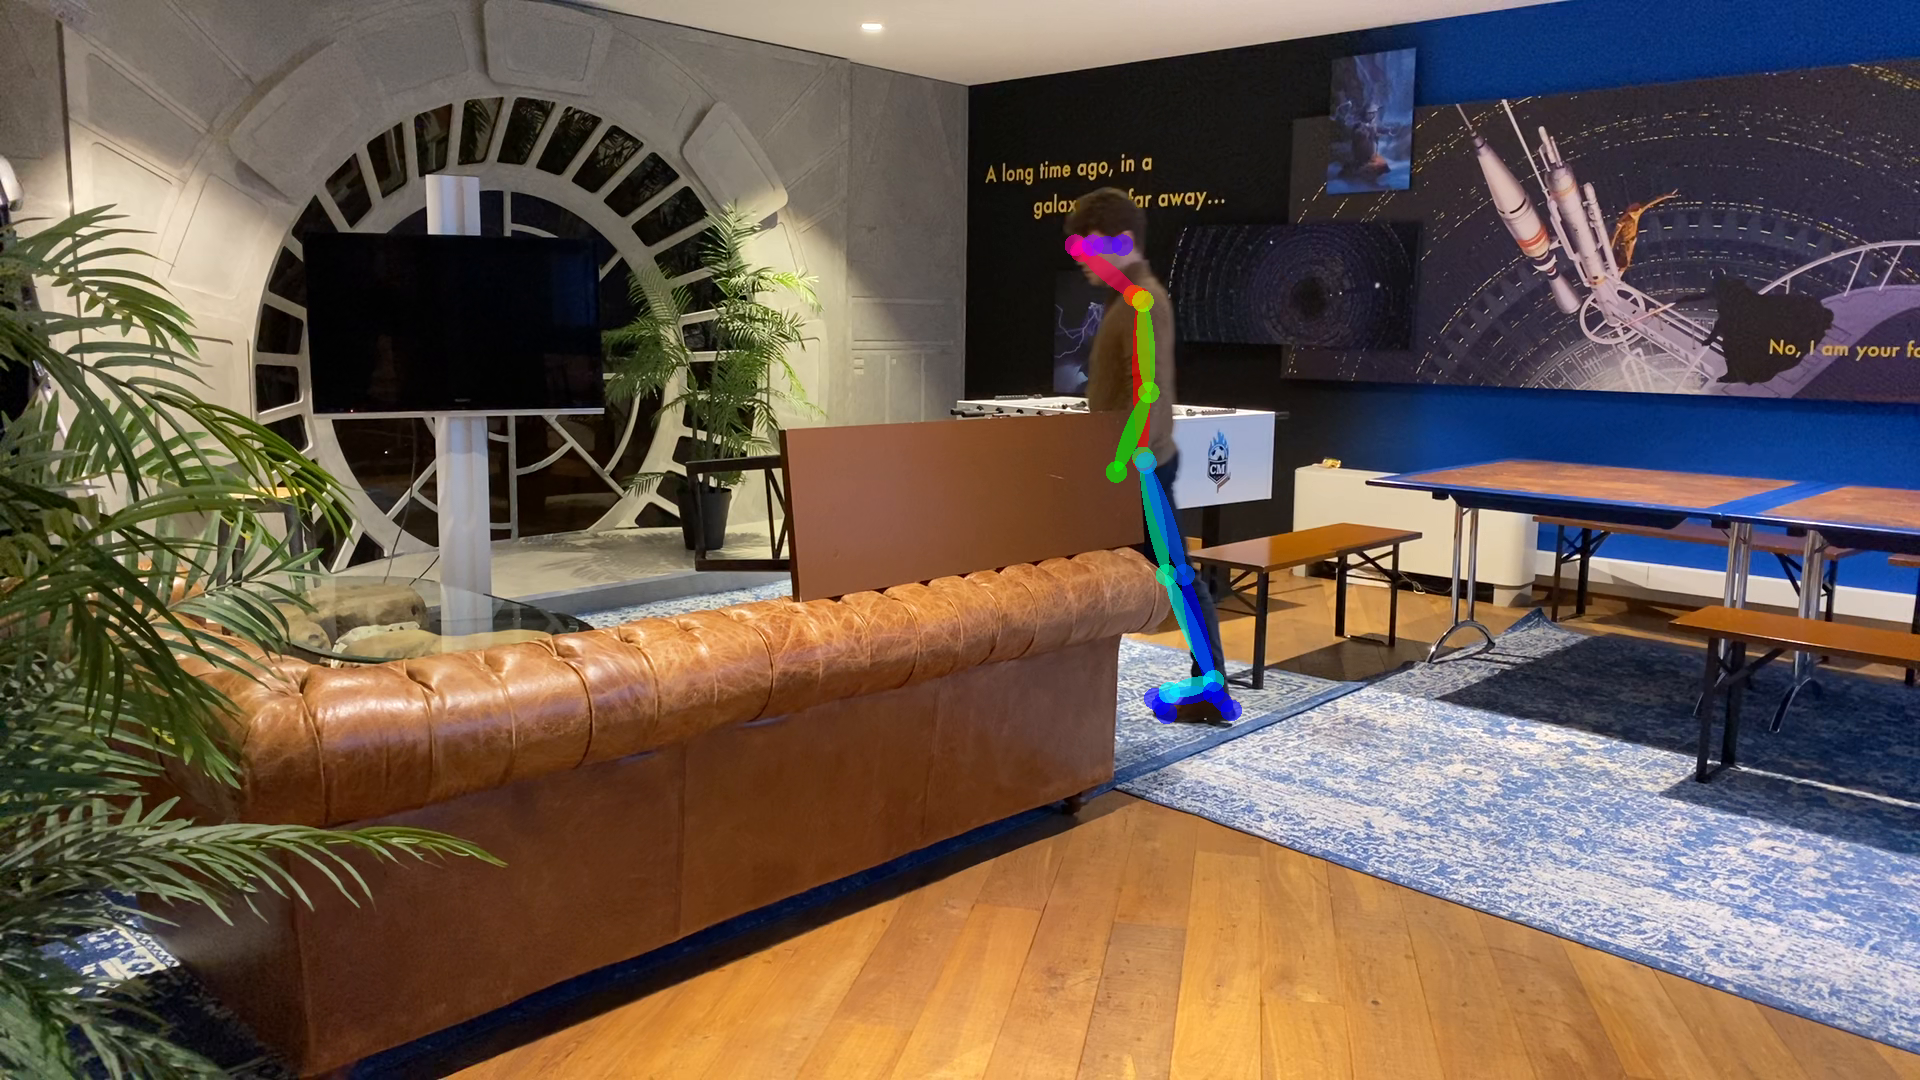
\includegraphics[width=0.3\textwidth]{Figures/humor/qualitative/bad/occluded_walking_failed/openPose.png}} 
    \hfil
    \subfloat[Stage 2]{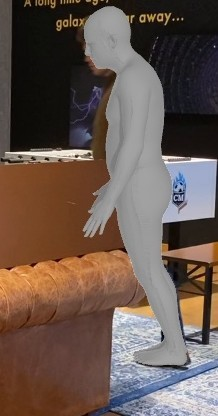
\includegraphics[width=0.3\textwidth]{Figures/humor/qualitative/bad/occluded_walking_failed/stage2.jpg}} 
    \hfil
    \subfloat[Stage 3]{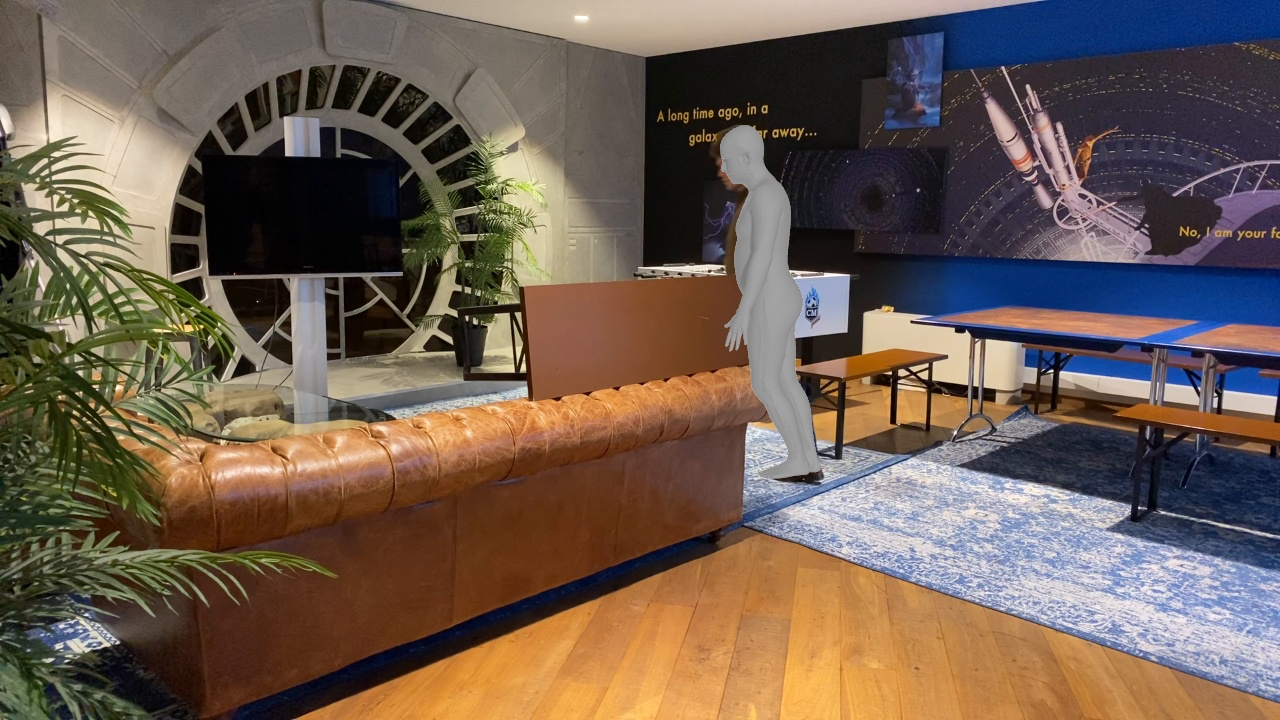
\includegraphics[width=0.3\textwidth]{Figures/humor/qualitative/bad/occluded_walking_failed/stage3.jpg}}
    \caption{Occluded walking failure point, 2 legs predicted instead of 1}
    \label{fig:humor_bad_occluded_walking}
\end{figure}

We also found that the choice of axis angle representation for various rotations led to the emergence of common known issue that arising from the discontinuities present in the representation \cite{aa_6d_angles}. The shortest path between certain angles in axis angle space can lead to a 360 degree rotation, as seen in \figref{fig:humor_bad_aa}, among other issues.

\begin{figure}[h!]
    \centering
    \subfloat[]{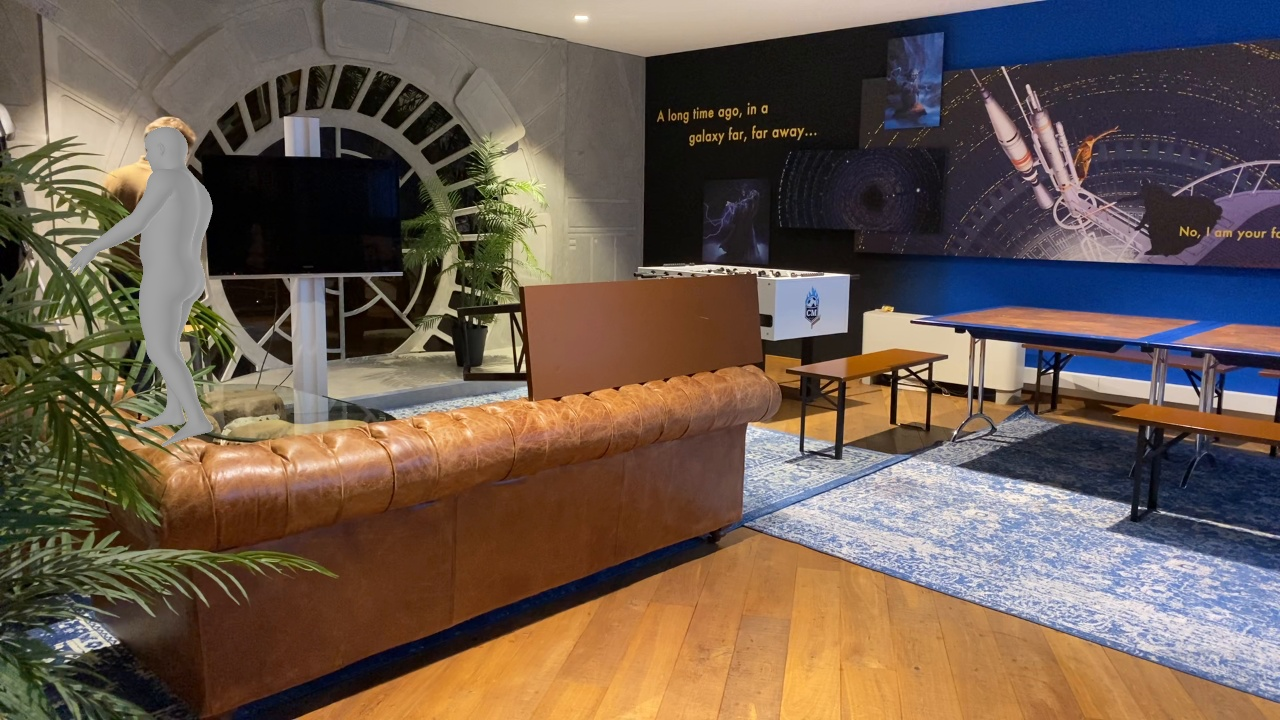
\includegraphics[width=0.3\textwidth]{Figures/humor/qualitative/bad/aa_issue/frame_00000331.jpg}}
    \hfil
    \subfloat[]{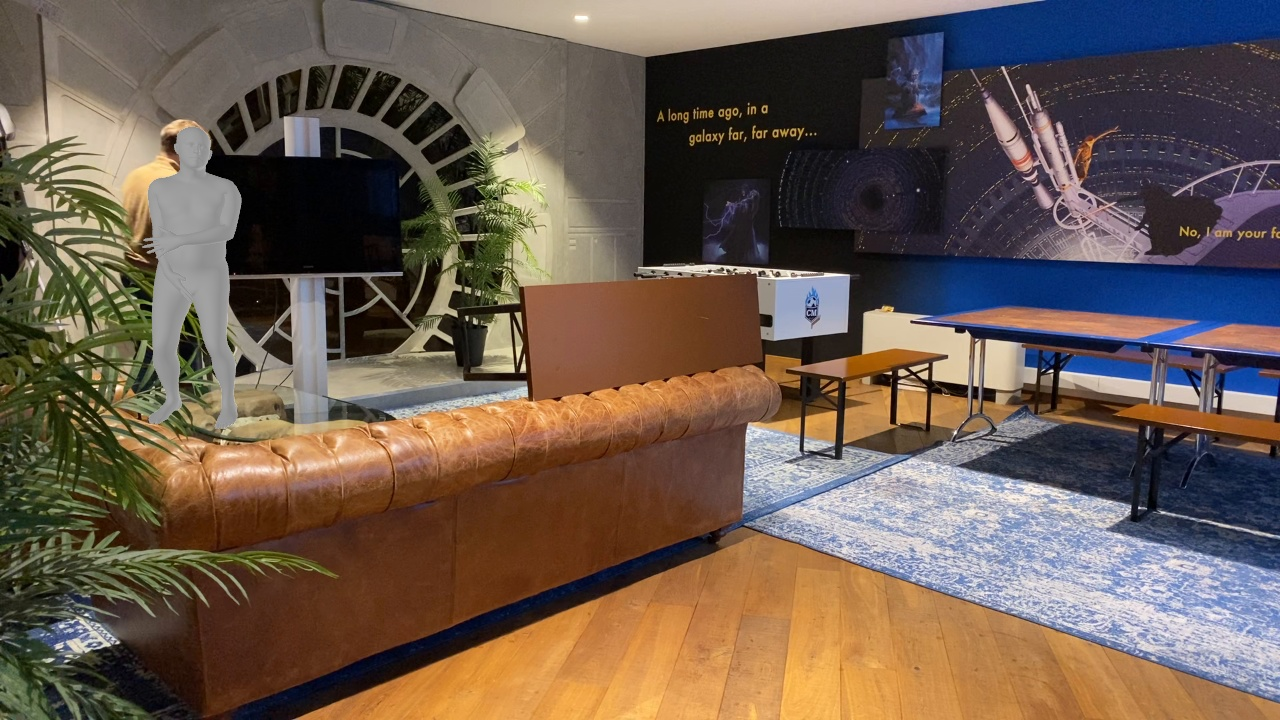
\includegraphics[width=0.3\textwidth]{Figures/humor/qualitative/bad/aa_issue/frame_00000336.jpg}} 
    \hfil
    \subfloat[]{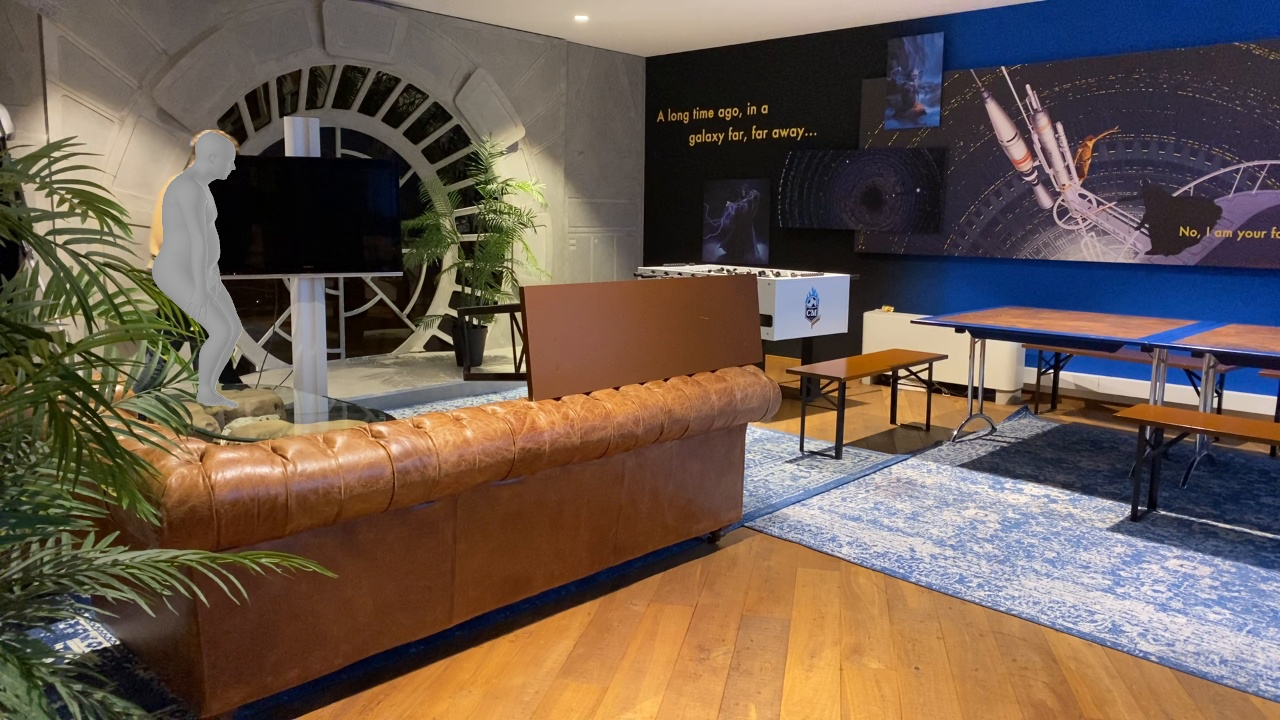
\includegraphics[width=0.3\textwidth]{Figures/humor/qualitative/bad/aa_issue/frame_00000342.jpg}}
    \caption{Axis angle issue: dubious rotations}
    \label{fig:humor_bad_aa}
\end{figure}

We found that the TestOps system would occasionally get itself into a tangle, as seen in \figref{fig:humor_bad_mess}, we assume due to the autogregressive nature resulting in a potentially catastrophic cumulation of errors, and found this happended most notably for a sequence containing someone rolling on the floor. It is interesting to note that these sorts of motions were not often, if ever, present in the training data.

\begin{figure}[h!]
    \centering
    \subfloat[OpenPose]{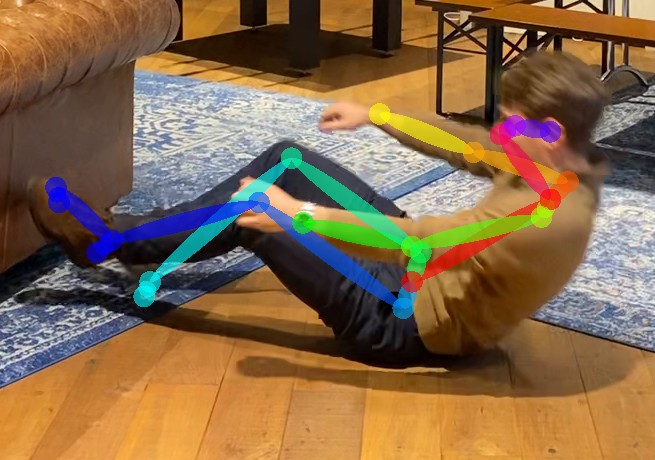
\includegraphics[width=0.3\textwidth]{Figures/humor/qualitative/bad/unrecoverable/openPose.png}} 
    \hfil
    \subfloat[Stage 2]{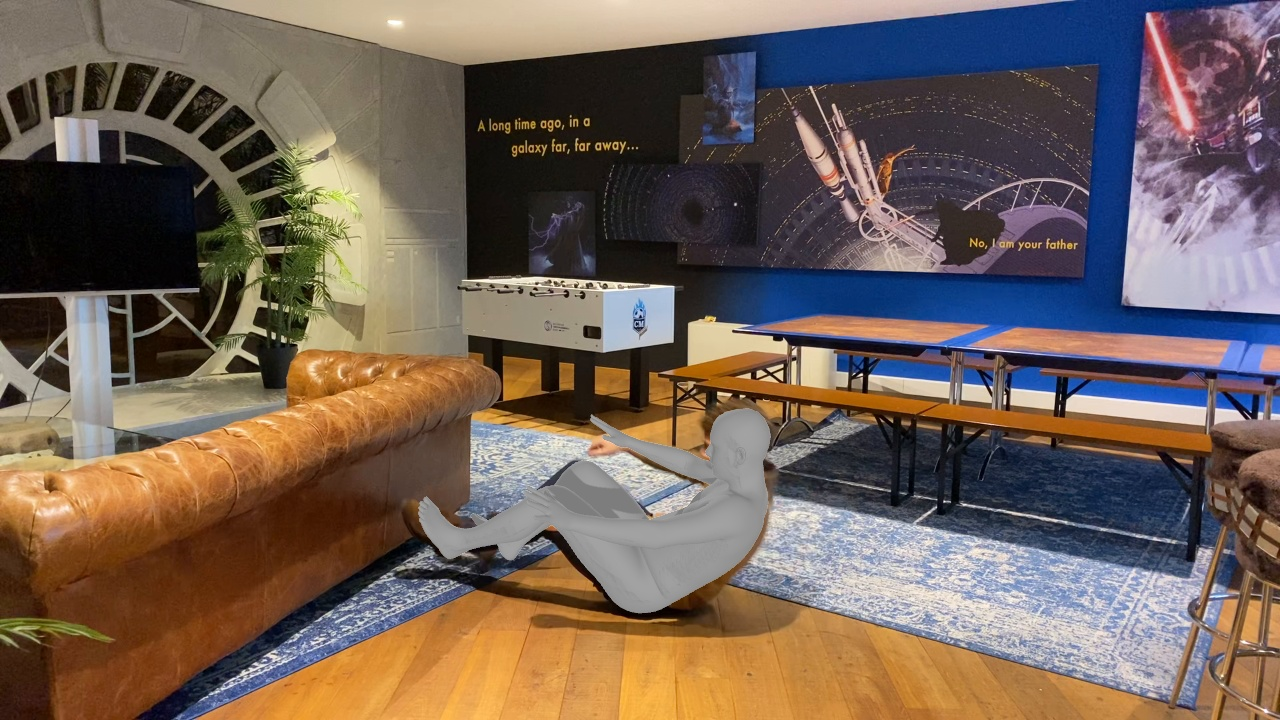
\includegraphics[width=0.3\textwidth]{Figures/humor/qualitative/bad/unrecoverable/stage2.jpg}} 
    \hfil
    \subfloat[Stage 3]{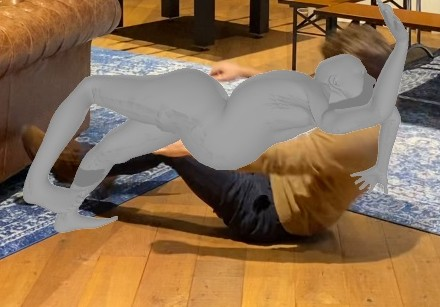
\includegraphics[width=0.3\textwidth]{Figures/humor/qualitative/bad/unrecoverable/stage3.jpg}}
    \caption{HuMoR in a tangle}
    \label{fig:humor_bad_mess}
\end{figure}

Next, we saw overly smoothed motion for certain clips, most notably for particularly stylised motion such as dancing.  We also found that if there is a single frame without Open Pose predictions then as of that frame the TestOps fails. Finally, and most importantly, we found that the TestOps was extremely slow. It took around 20mins per 2s clip, and that we could batch at most 4 2s clips together, so 20mins per 8s on a Nvidia GeoForce 1080ti with 11Gbs memory.

We concluded that there were a number of potential benifits, notably in occluded situations, and that many of the issues, including the axis angle representation issue, the dependence on humor, and smooth motion, have a good chance of being fixed with different design choices.  The glaring issue however was the unresonable amount of time the system took, rendering it unusable for our purposes as we wish the system to be close to real time.

\subsection{Profiling}
To investigate this speed issue, we profiled the code, as can be seen in \figref{fig:humor_profiling}. We found that the program spent 90\% of it's time in the Stage 3 optimiser closure, 56\% of it's time performing the backwards step and 32\% of it's time in the rollout function. Hence it was clear that the speed issue was due to the slow act of rolling out and the large computation necessary to perform the backwards step on the large computation graph resulting from the rollout.

\begin{figure}[h!]
    \centering
    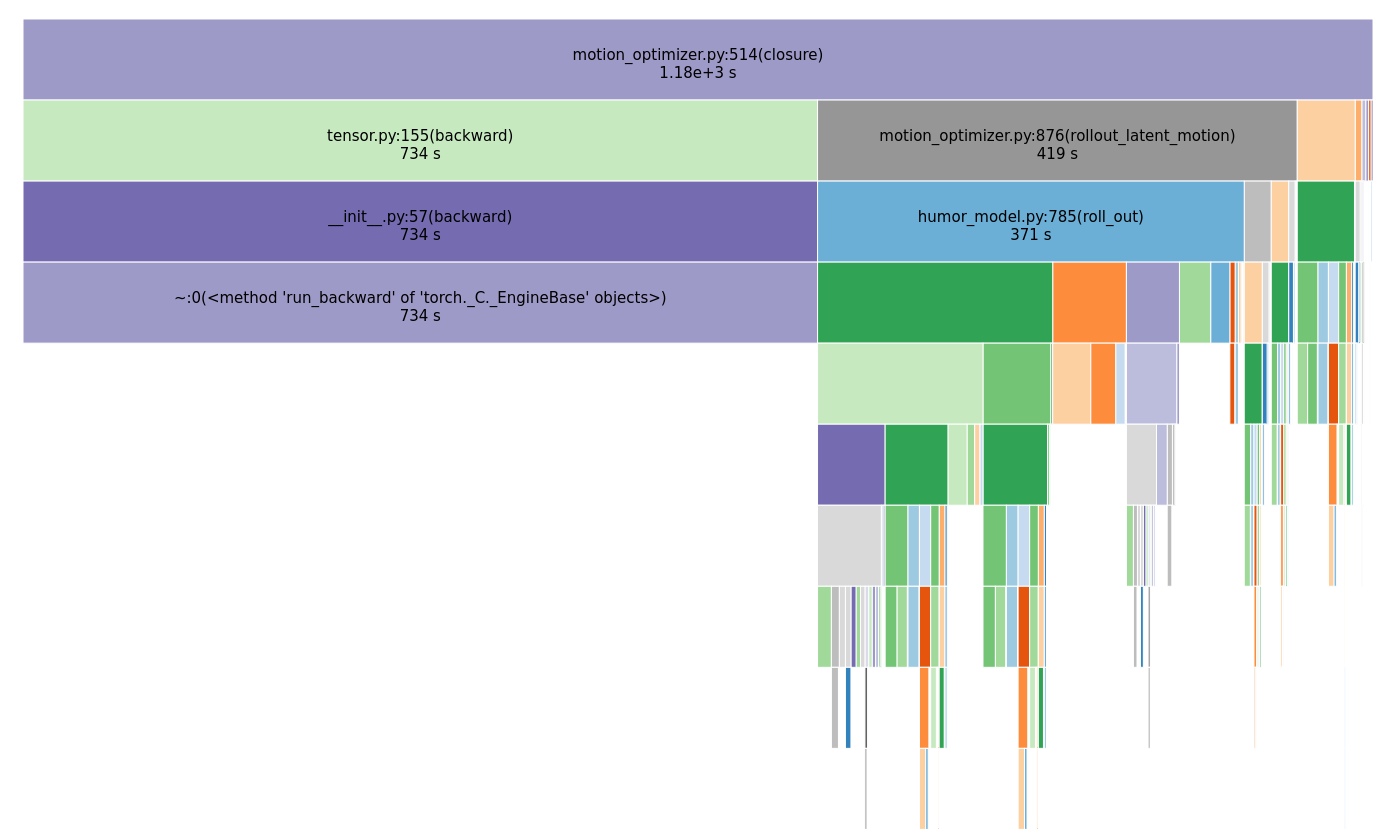
\includegraphics[width=1\textwidth]{Figures/humor/profiling/profiling.png}
    \caption{TestOps profiling}
    \label{fig:humor_profiling}
\end{figure}

\subsection{Conclusion}
We came to the final conclusion that the HuMoR motion model alongside the TestOps optimisation showed potential, but that it must be sped up before we can conclusively say if it is of particular use to us. We note that to speedup the method, we must primarily focus on improving/removing the rollout. Thus, in the next section, an attempt to speed up the TestOps is made.

\section{Improving HuMoR TestOps}
\label{sec:humor_improvement}

This section presents the attempt that was made at modify the TestOps of the HuMoR paper \cite{humor} in such a way that we attain comparable results but in a significantly shorter timespan.

\TODO{See if I have introduced the terms properly (decoded sequence, $x$'s, $x'$'s, etc.)}

\subsection{Speeding up the TestOps}

Realising that the main speed limitations are due to the concept of rollout over the entire sequence, we decided to break this long range dependence. Through short overlapping rollouts, it is possible to acheive more parrallelisation and smaller computation graphs, and our intuition suggests that the need for such a large context window is not necessary, that only a small number of autoregressed frames are needed to be able to propagate information sensibly and to get meaningful gradients. Anecdotaly, it would seem intuitive that if a video contains sitting, then walking, then sitting again, the second act of sitting would not depend in on the early act of sitting, hence rolling out over the whole sequence seems unnecessary.

The HuMoR TestOps rollout is presented graphically in \figref{fig:humor_rollout_graph}. $x$ is the state, and $z$ are the latent variables, the optimised variabels are highlighted in pink, and the losses are coloured, gray x's indicate they are calculated during the optimisation from the optimised variables. As can be seen, first all the states are autoregressed from the initial state and the latent variables, and then the losses are applied. This can be seen to result in very long range dependencies in the computation graph, thus making the gradients time consuming to calculate. 

\begin{figure}[h!]
    \centering
    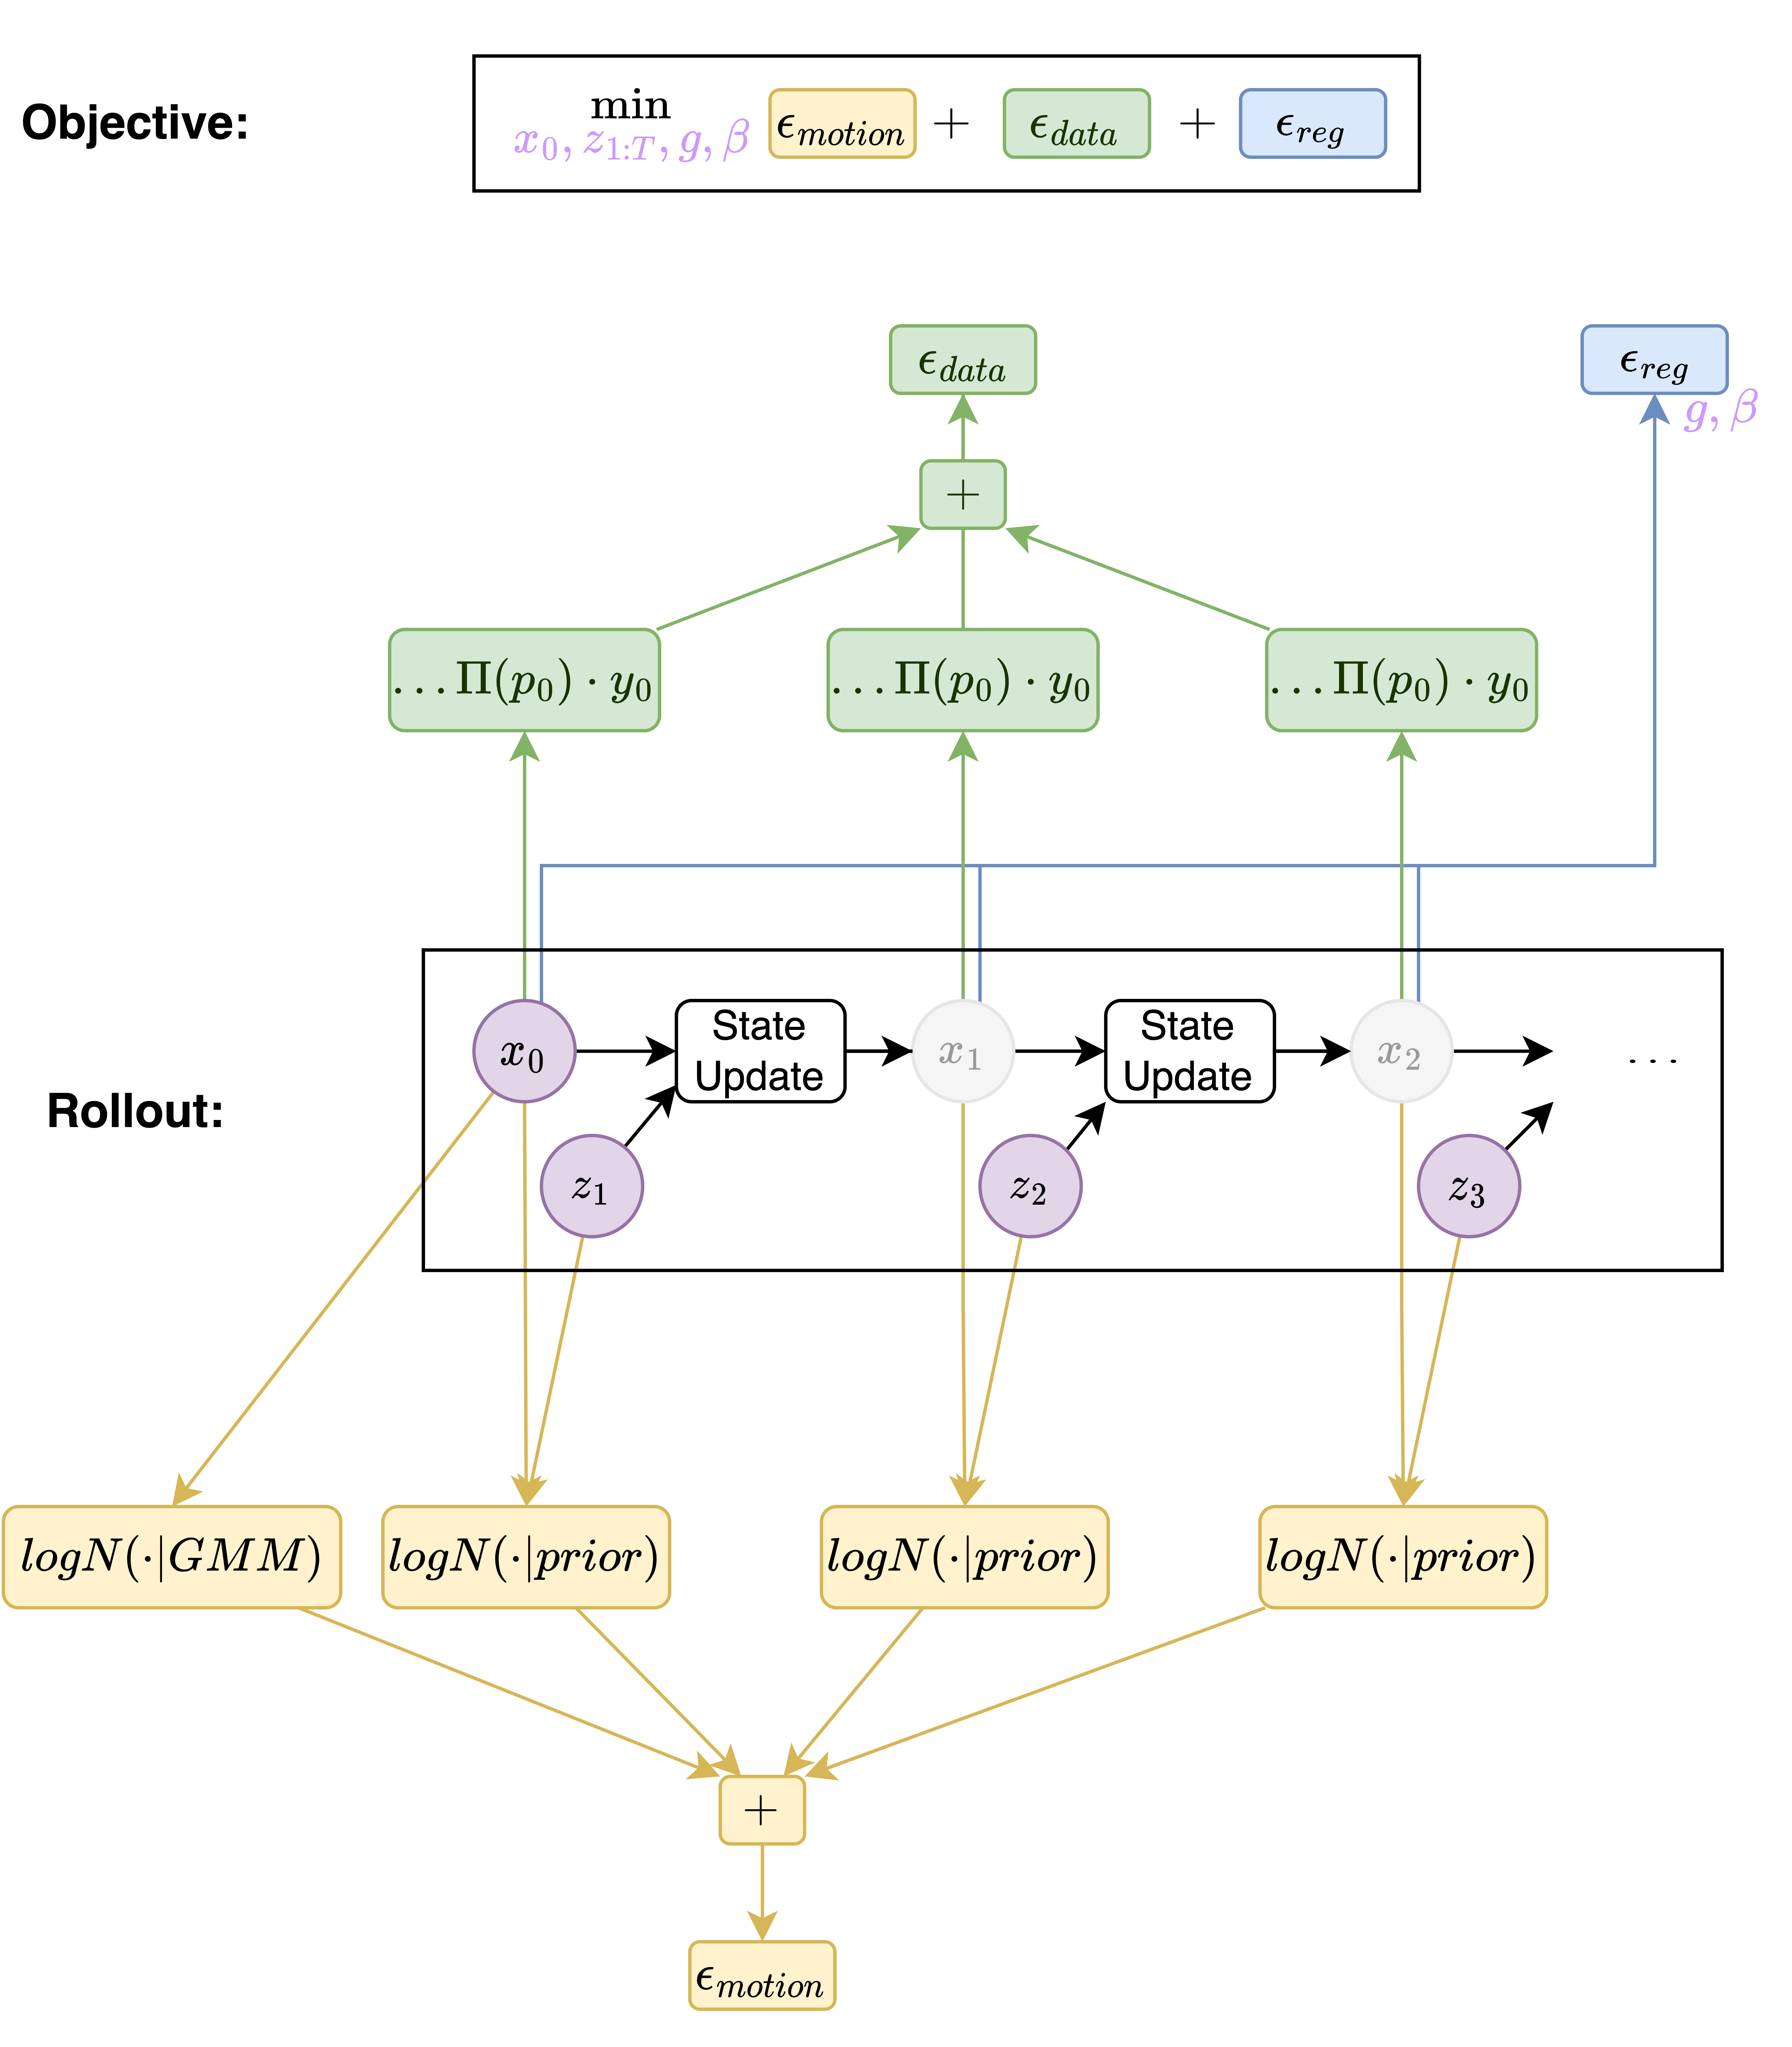
\includegraphics[width=1\textwidth]{Figures/humor/improvement/computation_graph_humor.png}
    \caption{TestOps Computation Graph}
    \label{fig:humor_rollout_graph}
\end{figure}

\TODO{Update \figref{fig:dimm_rollout_graph} and remove the 'NEW' norm, labels on green loss, and potentially red loss?}

The most obvious way to break this autogregression is to maintain and optimise a separate sequence of $x$'s, updating this seperate sequence with reference to the $x'$'s decoded from the latent variables as in \figref{fig:dimm_rollout_graph}. We can take into account the decoded $x'$'s in several manners:
\begin{itemize}
    \item Copy over
    \begin{itemize}
        \item Directly replace the optimised sequence of $x$'s with the decoded $x'$'s.
    \end{itemize}
    \item Blend
    \begin{itemize}
        \item Perform a weighted addition of the optimised $x$'s and decoded $x'$'s.
    \end{itemize}
    \item Loss term
    \begin{itemize}
        \item Add a loss term on the difference between the optimised $x$'s and decoded $x'$'s. 
    \end{itemize}
\end{itemize}

All decoding steps can now be performed in parrallel, rather than sequentially, which greatly reduces the computation time. 

\begin{figure}[h!]
    \centering
    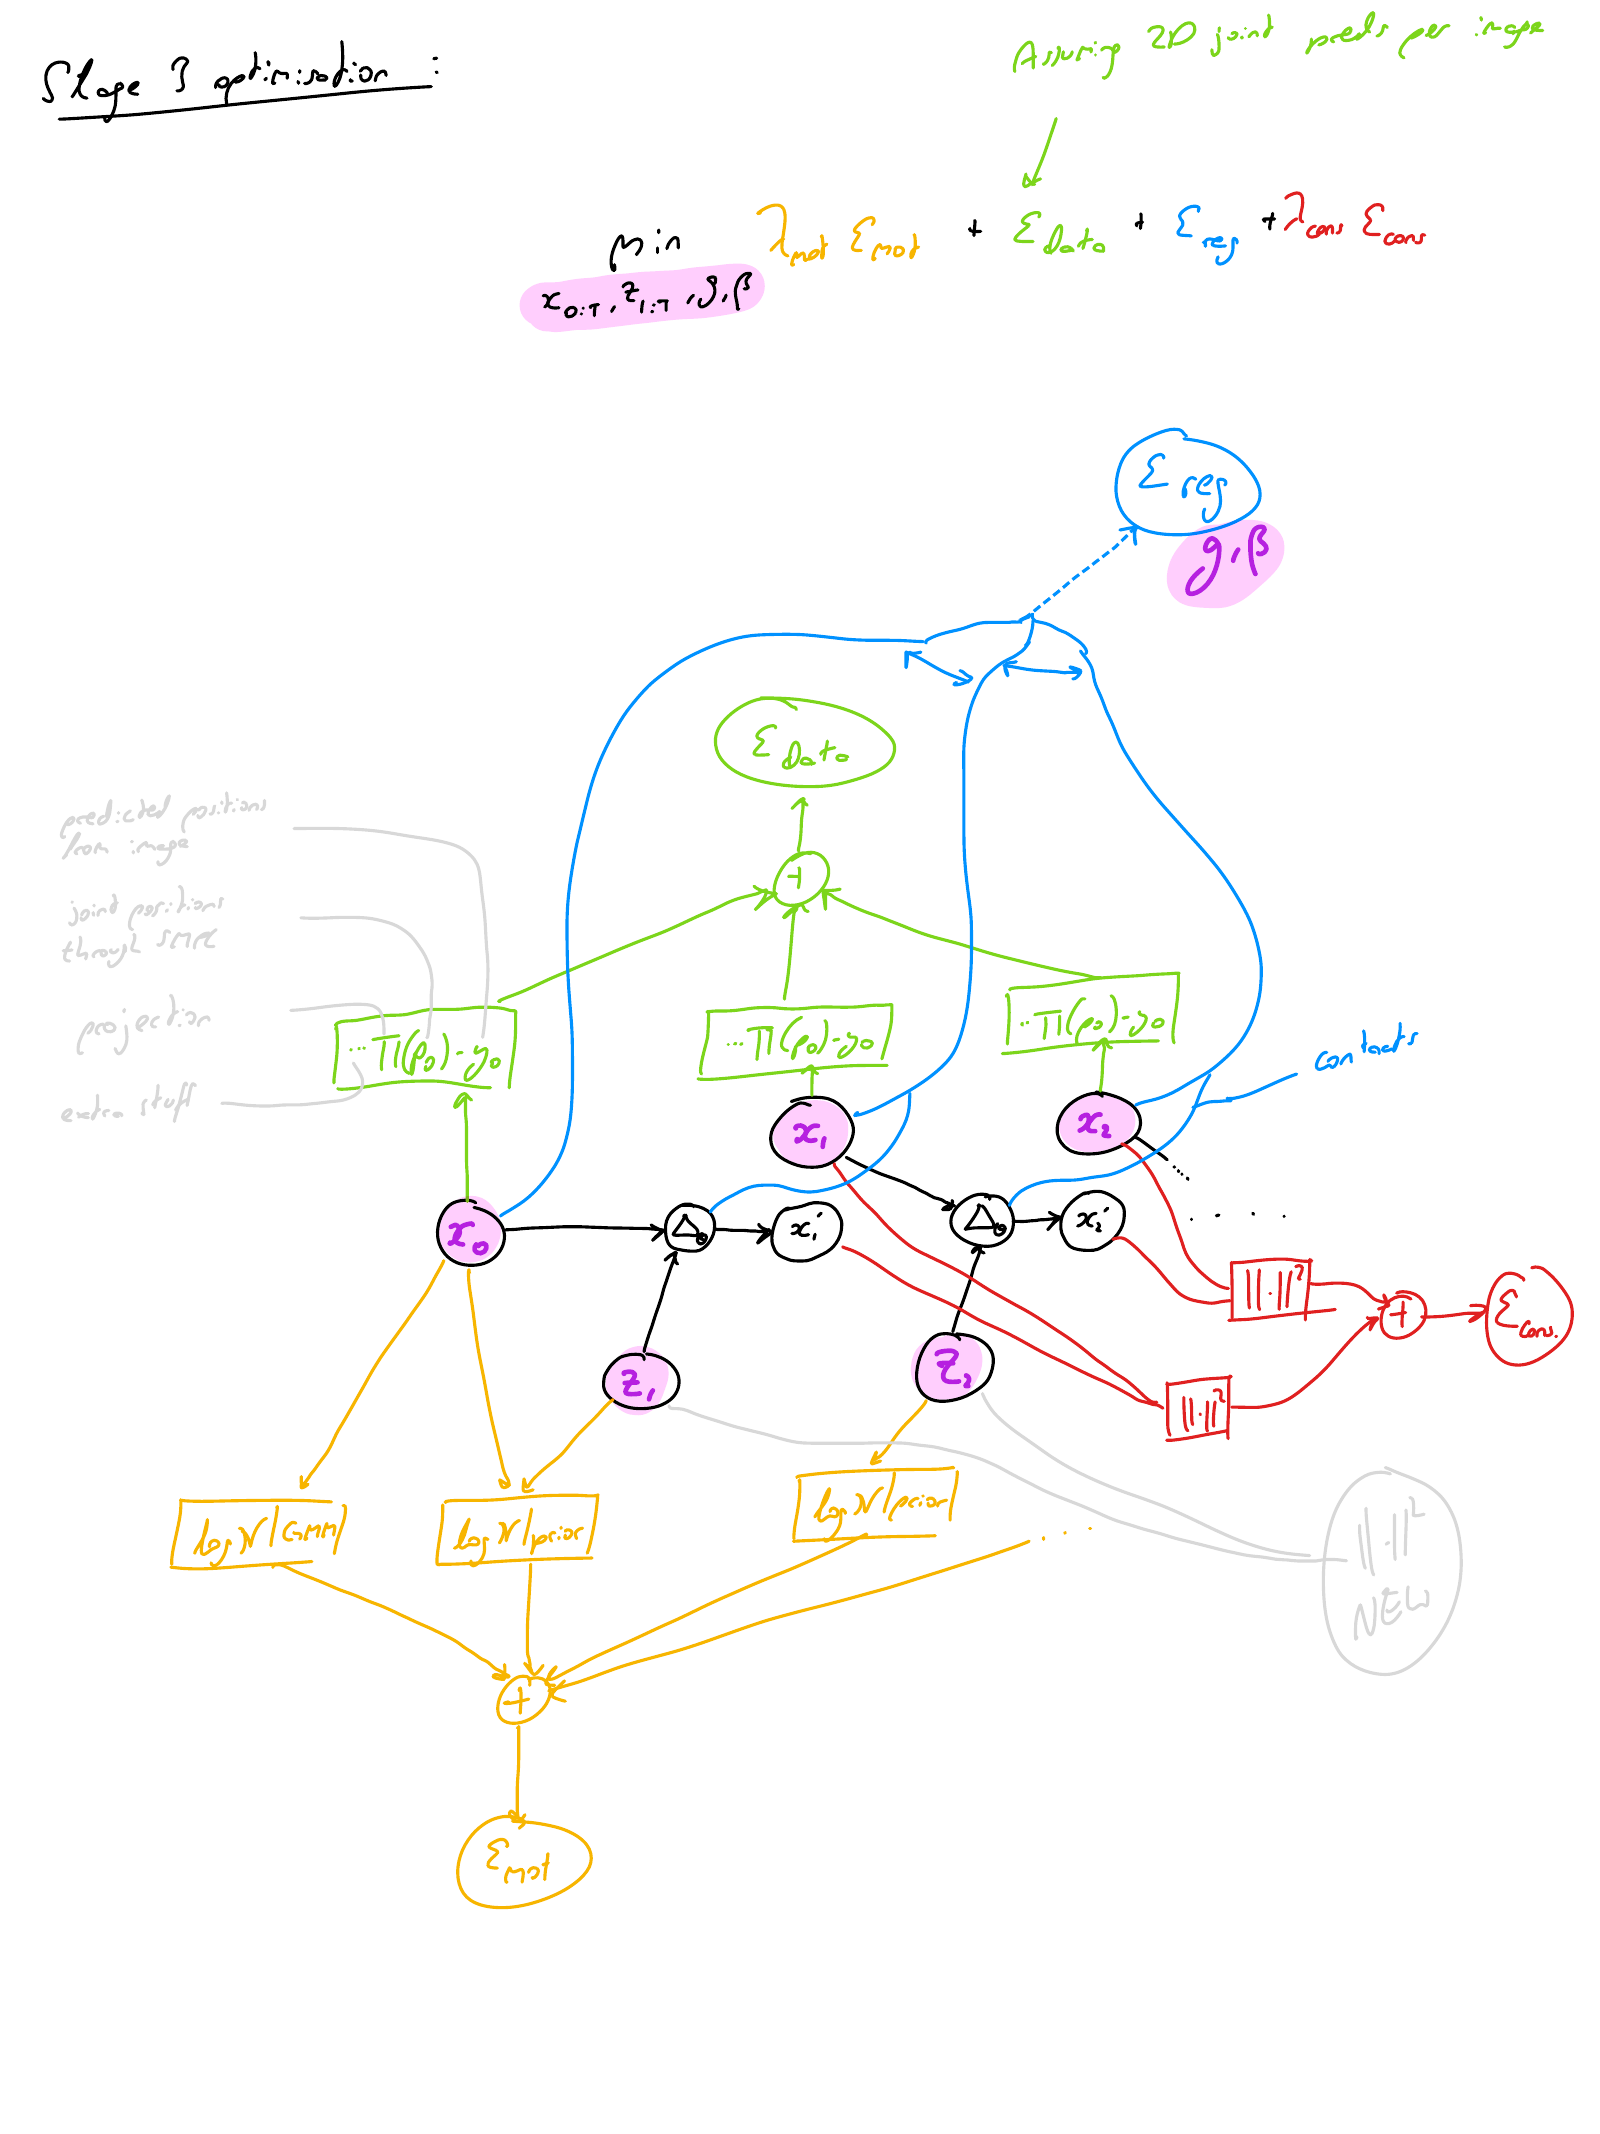
\includegraphics[width=1\textwidth]{Figures/humor/improvement/computation_graph_dimm.png}
    \caption{Decoupled Computation Graph}
    \label{fig:dimm_rollout_graph}
\end{figure}

This new method also allows us to experiment with different amounts of rollout. We can once again decode the decoded sequence of $x'$'s to get $x''$, and so on and so forth. These extra sequences are all decoded with the same latent variables thus the updates to the latent variables will take into account the losses on all the decoded sequences. Graphically this can be seen in \figref{fig:dimm_decoded_sequences}, where each next line .
\TODO{describe the figure better}

\begin{figure}[h!]
    \centering
    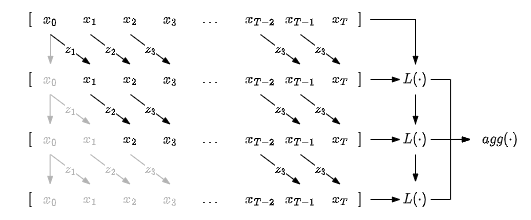
\includegraphics[width=1\textwidth]{Figures/humor/improvement/Rollout_overlap.png}
    \caption{Decoded sequences}
    \label{fig:dimm_decoded_sequences}
\end{figure}

The information contained in each $x$ can flow forwards through the short range rollouts, and over the iterations of the optimiser. Note however that the information flow will be slower than the HuMoR TestOps, as in the TestOps all subsequent $x$'s are regressed from the initial $x_0$.
In the HuMoR TestOps information can flow backwards from any future frame's $x$ in one update through the gradients, as all $x$'s are linked in the computation graph through the auto-regression (though our intuition suggests that the information does not actually need to flow so far, as previously discussed). In the new method however, the information flow will be much more limited, as the rollouts will be significantly shorter, though again the information should flow through the iterations fo the optimiser.

\subsection{Implementation notes}

A number of issues were encountered during the implementation that are worth mentioning. After implementing the new method, attempts were made to get the optimiser to produce sensible results. The general approach was to use a small number of losses, so as to get a better intuition of each loss, with the goal of better understanding how to balance the losses in the optimiser, but some errors in individual losses were encountered.

Firstly, as expected, the Axis-Angle representation became a problem. When running through functions to convert to root-local reference frame for the HuMoR model for decoding (as it operates on said reference frame), and then back to world reference frame for the opftimiser, the Axis-Angle vector flipped direction. Though the flipped vector still represented the same rotation, the angle representations of the same angle in the optimised sequence of $x$'s and the decoded sequence of $x'$'s were different, hence encorporating the information from decoded sequence cause the angle to move somewhere between the two flipped values which was no longer a sensible angle representation, thus resulting in root flips and other strange effects.

Secondly, an issue due to the SMPL model was found. When using a 2d reprojection loss (comparing the projected SMPL joints to the OpenPose 2d predictions) on a sequence where only the left arm and face had any OpenPose predictions, the legs were being moved by the optimiser. This was wrong as there were only losses on the arm and face joints, hence no gradients should flow to the legs. It was eventually found that the skinning weights of the SMPL model \cite{SMPL} contain spurious long range connections. 3\% of the LBS (linear blend skinning) weights in the SMPL model are non-zero but less than $1e-2$, which seems rather too low to have any meaningful effect on the skinning, but which allows for spurious gradients to flow. \\
For the comparison to the OpenPose predictions the OpenPose skeleton must be obtained from the SMPL mesh. Certain joints are regressed, other are simply taken directly as vertices from the mesh, as in the case of the nose joint in the OpenPose skeleton which is taken to be vertex 332 \cite{SMPL_op_joints}. We noted that this vertex 332 is skinned $99.8\%$ by the 'head' joint, but also $0.2\%$ by the right hip, left knee and right knee. This issue was solved by pruning all weights below 1e-2. It is interesting to note that there are known spurious connections in the SMPL blend shapes \cite{STAR}, but that we have found no reference to spurious connections in the LBS weights.

\subsection{Experiments}

% c.f Current_experiments.md for more details
\TODO{explain why the initial rollout was bad, and the compounding of errors forward}
\TODO{maybe we should discuss more in the humor investagtion section about the bad initial rollout}
\TODO{Check everything is explicitely named, e.g have a graphic clearly naming the optimised x's and the decoded x's, and what the z's are}

To begin with, we looked into the initial $z$'s that were obtained from projecting the Stage 2 results through the HuMoR encoder. We found that in occluded situations these $z$'s encode a sitting motion without any optimisation as seen in \figref{fig:humor_stage_2_rollout_sitting}, that simply the projection leads them to encode the necessary occluded motion. However we note that when autoregressively rolled out over a longer sequence the results, in \figref{fig:humor_stage_2_rollout_deviation}, deviate largely from the initial sequence of $x$'s seen in \figref{fig:humor_stage_2}. This shows us that though the initial $z$'s encode some sensible motion locally, and can be used to accurately recover the next frame, when they are chained together small deviations from the $x$ motion accumulate to create an overall deviation. For example if the arm is moved slightly too much by a single $z$, then all the future frames will have the arm in slightly the wrong position, and multiple $z$'s are wrong in the same direction, then the arm will raise up. This deviating sequence is the initial starting rollout in the Stage 3 of the HuMoR TestOps in which the rollout is optimised, though it seems unfortunate to us that from a sensible sequence of $x$'s obtained from Stage 2 we get such a bad sequence through the autoreggresive rollout. We do however note that though while this starting point represents a sequence that deviates largely, the $z$'s might not need to move so far to avoid the accumulation effect. The intuition in our case was that we are starting from some sensible $x$'s and $z$'s, and therefore that it should be possible to refine the $x$'s by take into account the HuMoR model through the $z$'s whilst updating the $z$'s. 

\begin{figure}[h!]
    \centering
    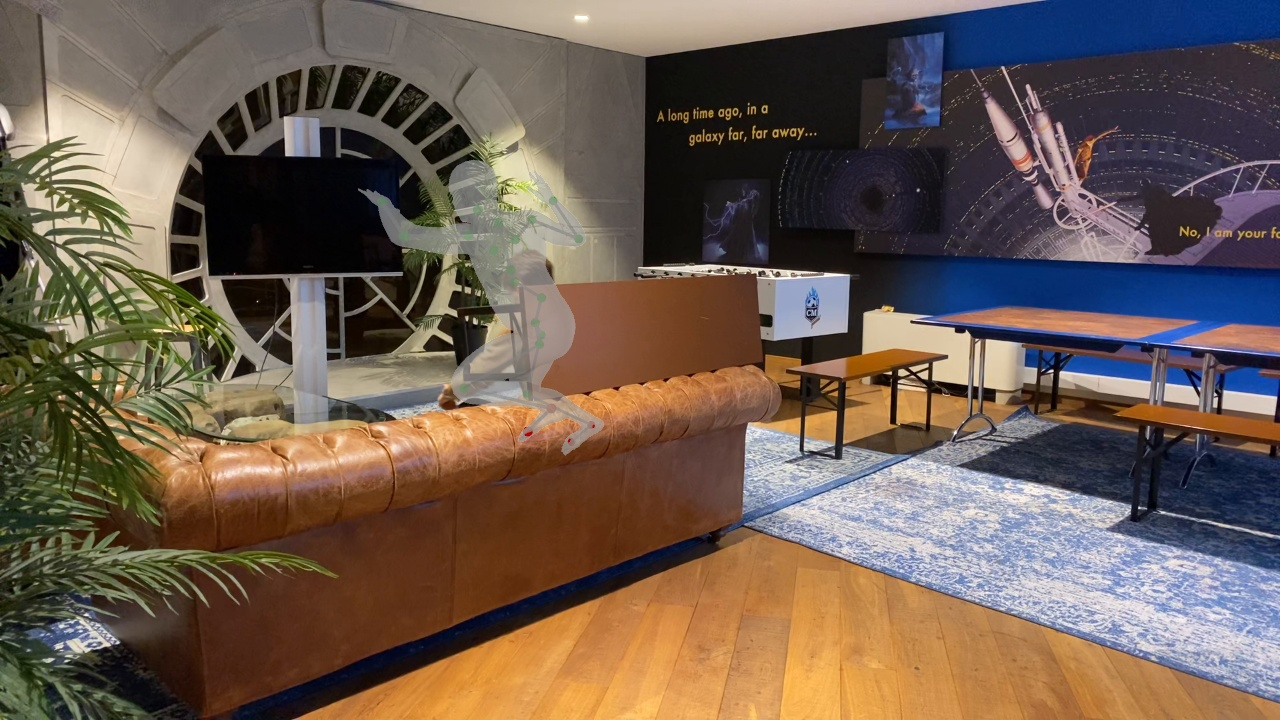
\includegraphics[width=1\textwidth]{Figures/humor/improvement/Rollout_stage_2/sitting_clip/rollout_sitting_example/frame_00000078.jpg}
    \caption{Stage2 $z$'s encode a sitting motion}
    \label{fig:humor_stage_2_rollout_sitting}
\end{figure}


\begin{figure}[h!]
    \centering
    \subfloat[]{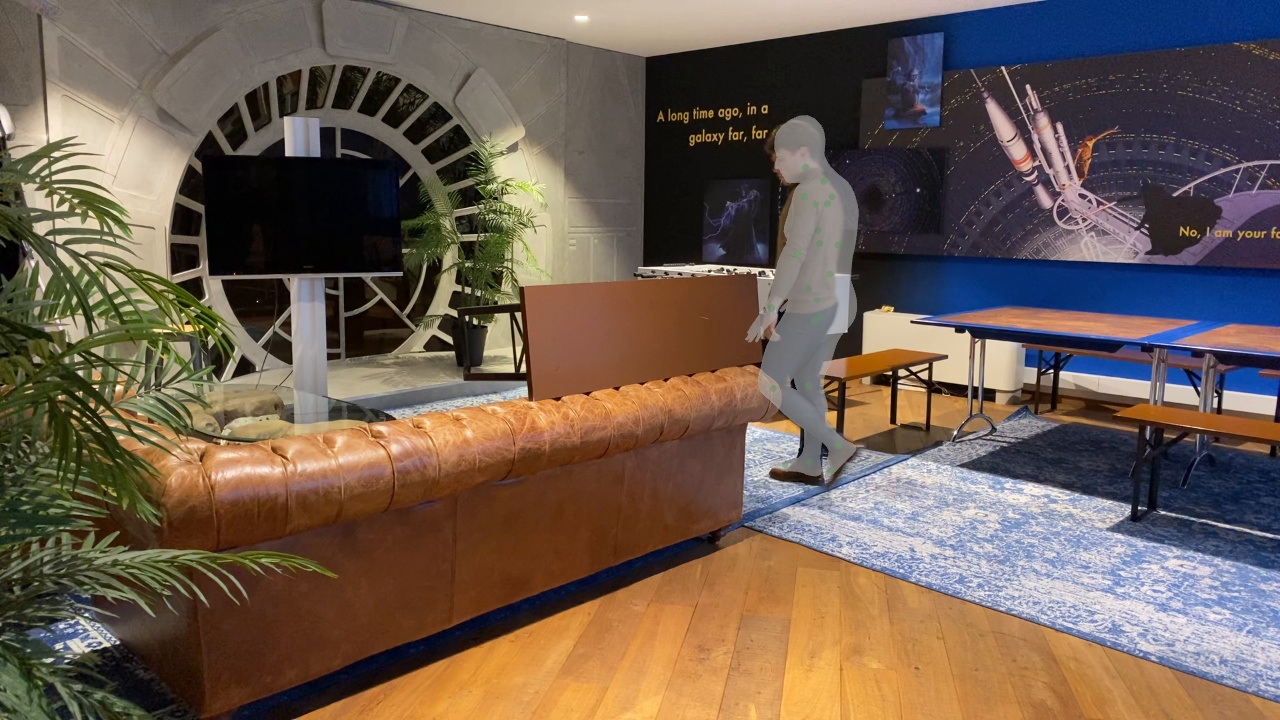
\includegraphics[width=0.3\textwidth]{Figures/humor/improvement/Rollout_stage_2/sitting_clip/stage2/frame_00000099.jpg}} 
    \hfil
    \subfloat[]{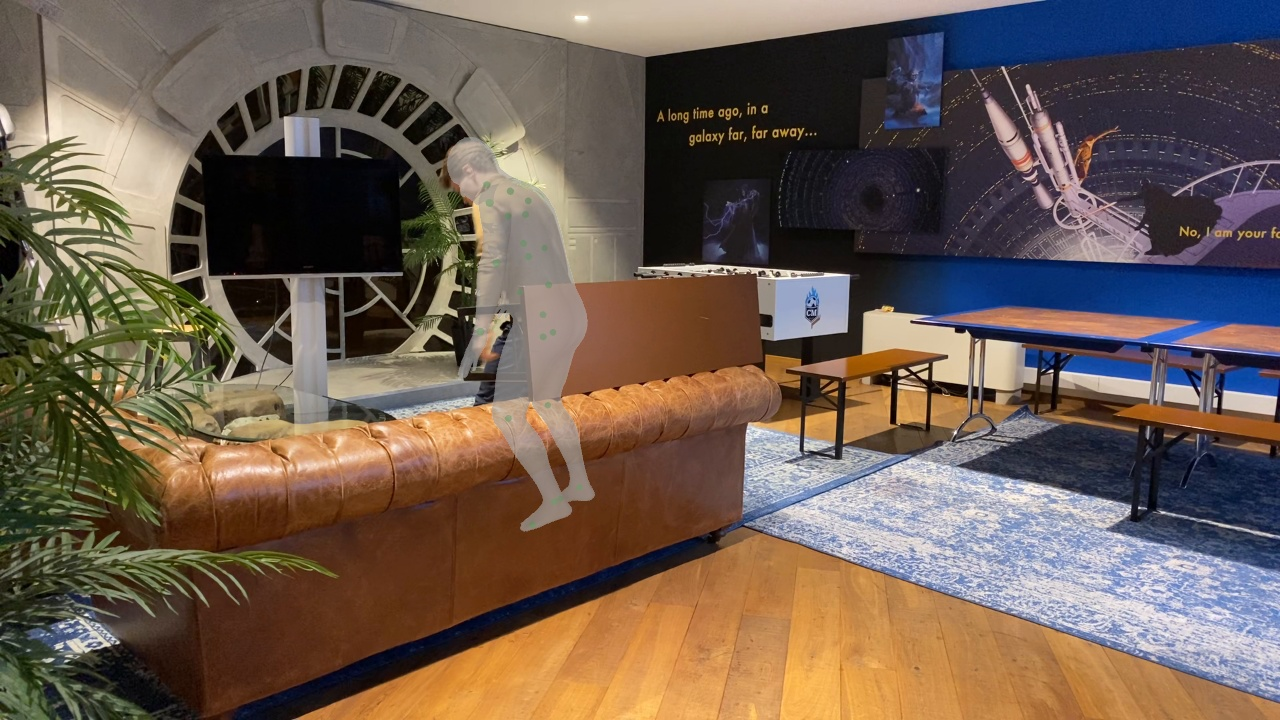
\includegraphics[width=0.3\textwidth]{Figures/humor/improvement/Rollout_stage_2/sitting_clip/stage2/frame_00000149.jpg}} 
    \hfil
    \subfloat[]{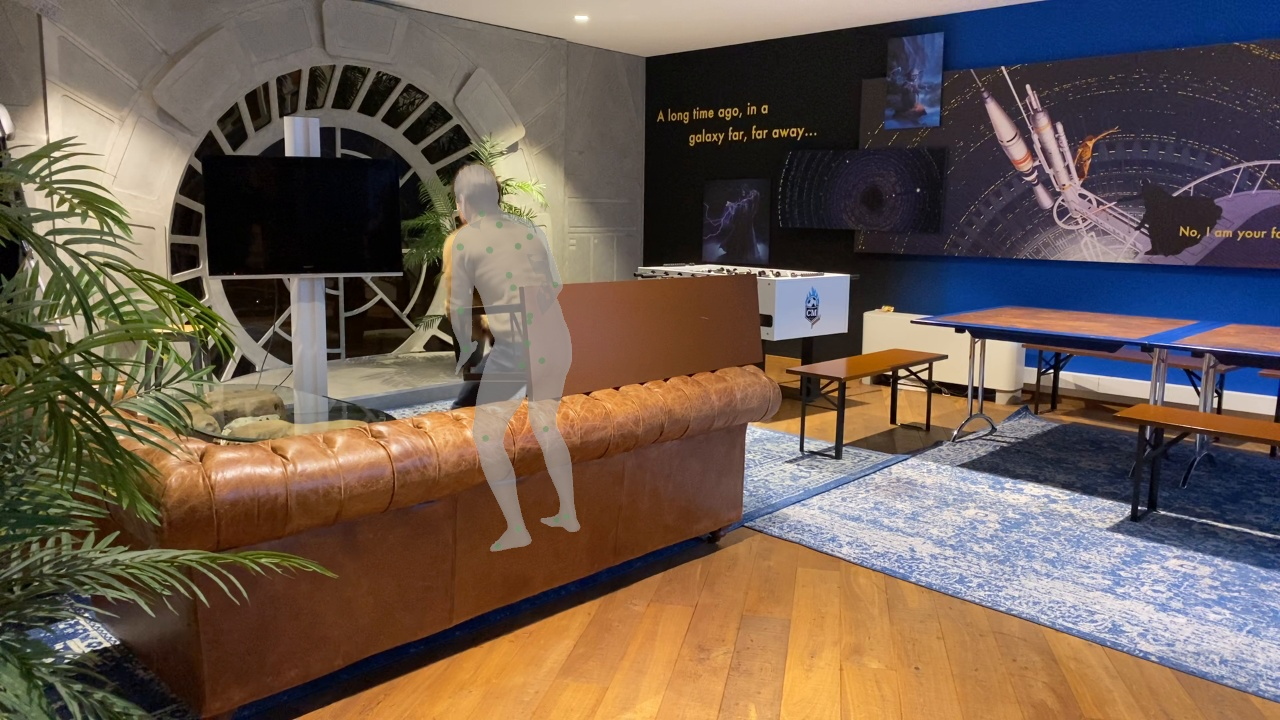
\includegraphics[width=0.3\textwidth]{Figures/humor/improvement/Rollout_stage_2/sitting_clip/stage2/frame_00000219.jpg}}
    \hfil
    \subfloat[]{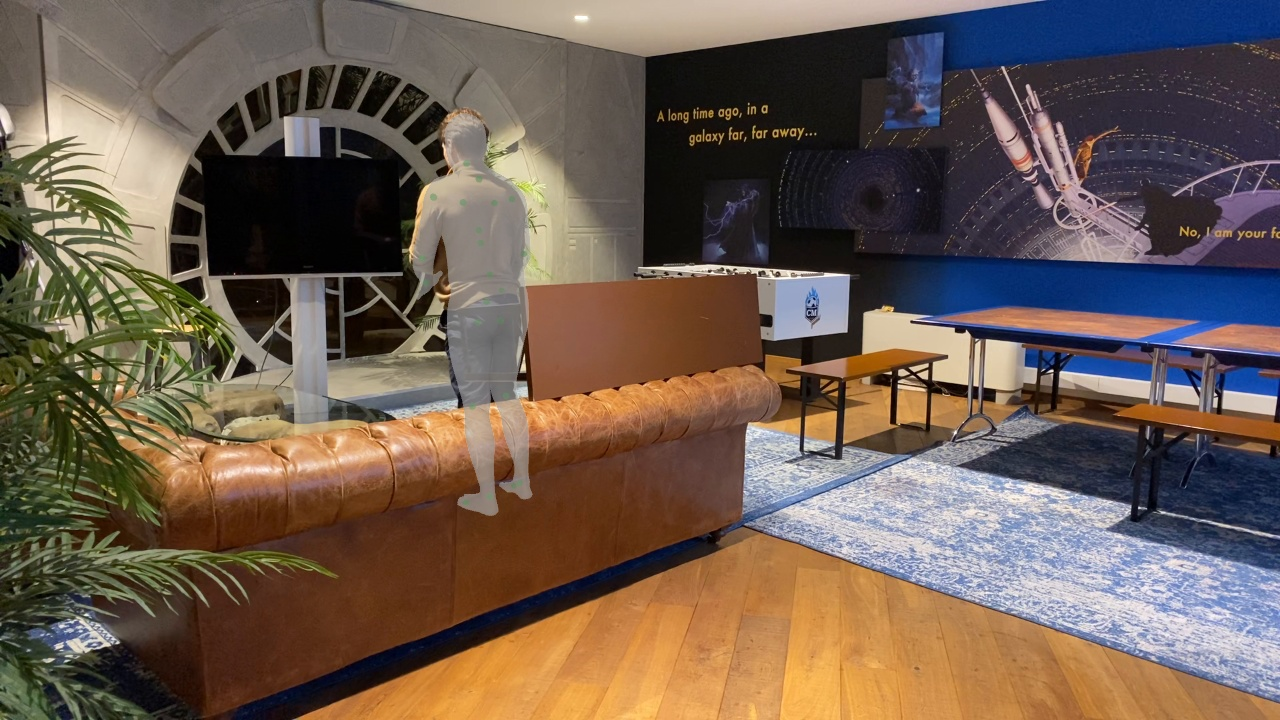
\includegraphics[width=0.3\textwidth]{Figures/humor/improvement/Rollout_stage_2/sitting_clip/stage2/frame_00000239.jpg}}
    \caption{Stage 2 $x$'s}
    \label{fig:humor_stage_2}
\end{figure}

\begin{figure}[h!]
    \centering
    \subfloat[]{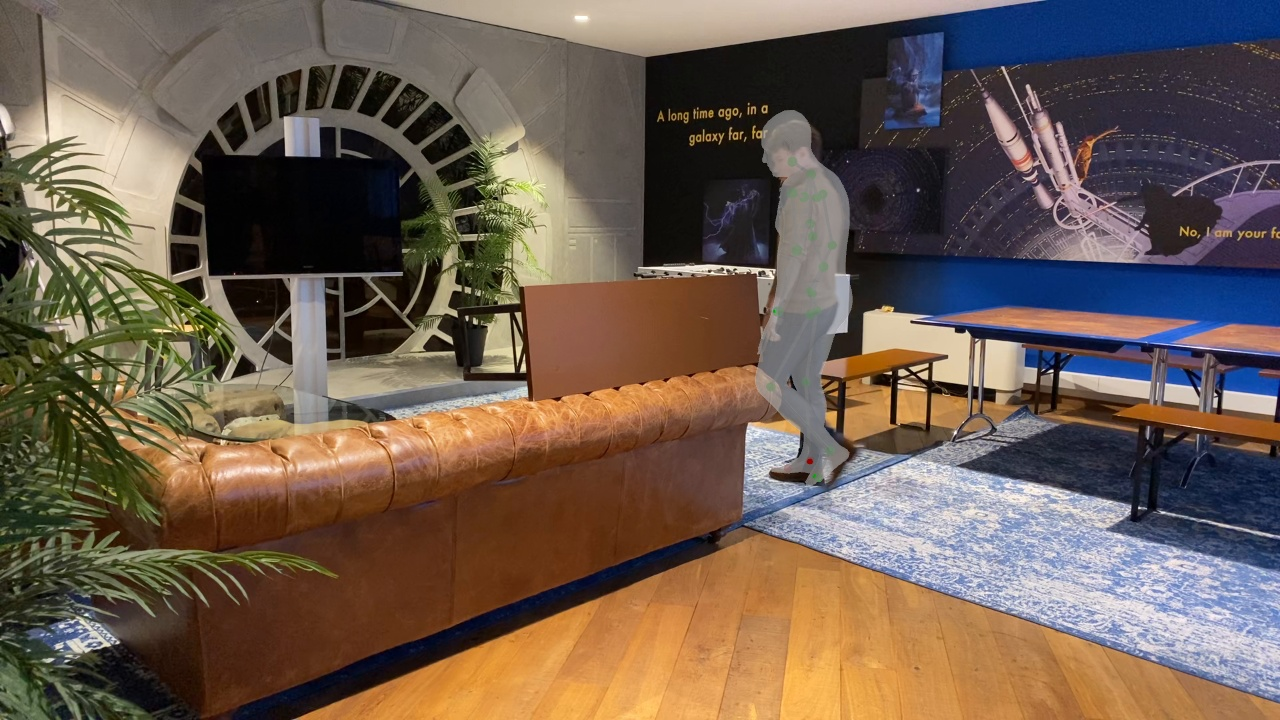
\includegraphics[width=0.3\textwidth]{Figures/humor/improvement/Rollout_stage_2/sitting_clip/rollout/frame_00000010.jpg}} 
    \hfil
    \subfloat[]{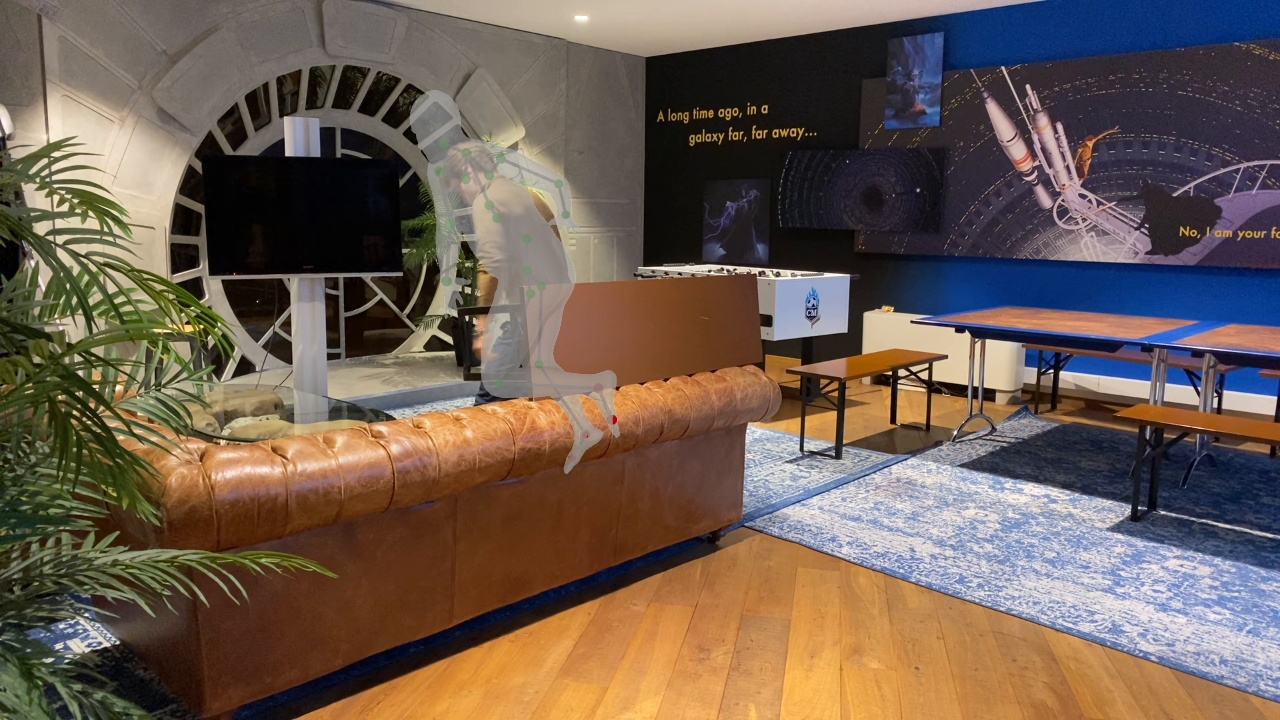
\includegraphics[width=0.3\textwidth]{Figures/humor/improvement/Rollout_stage_2/sitting_clip/rollout/frame_00000060.jpg}} 
    \hfil
    \subfloat[]{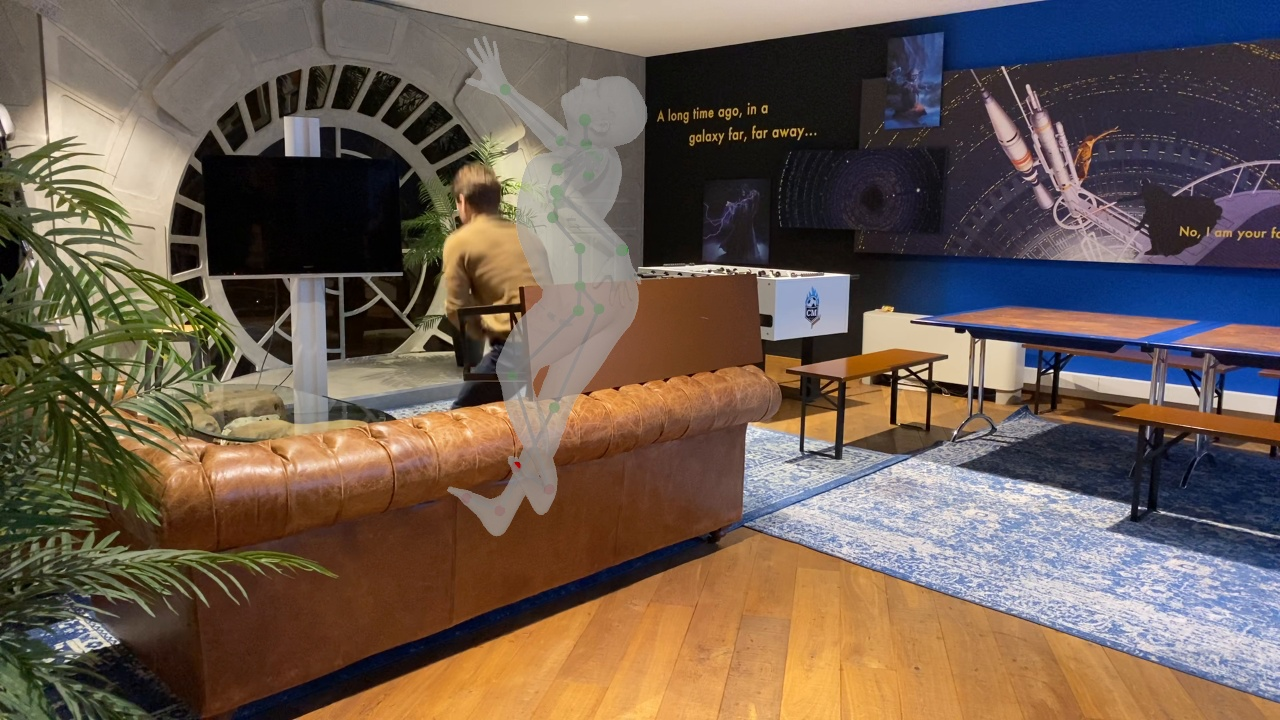
\includegraphics[width=0.3\textwidth]{Figures/humor/improvement/Rollout_stage_2/sitting_clip/rollout/frame_00000130.jpg}}
    \hfil
    \subfloat[]{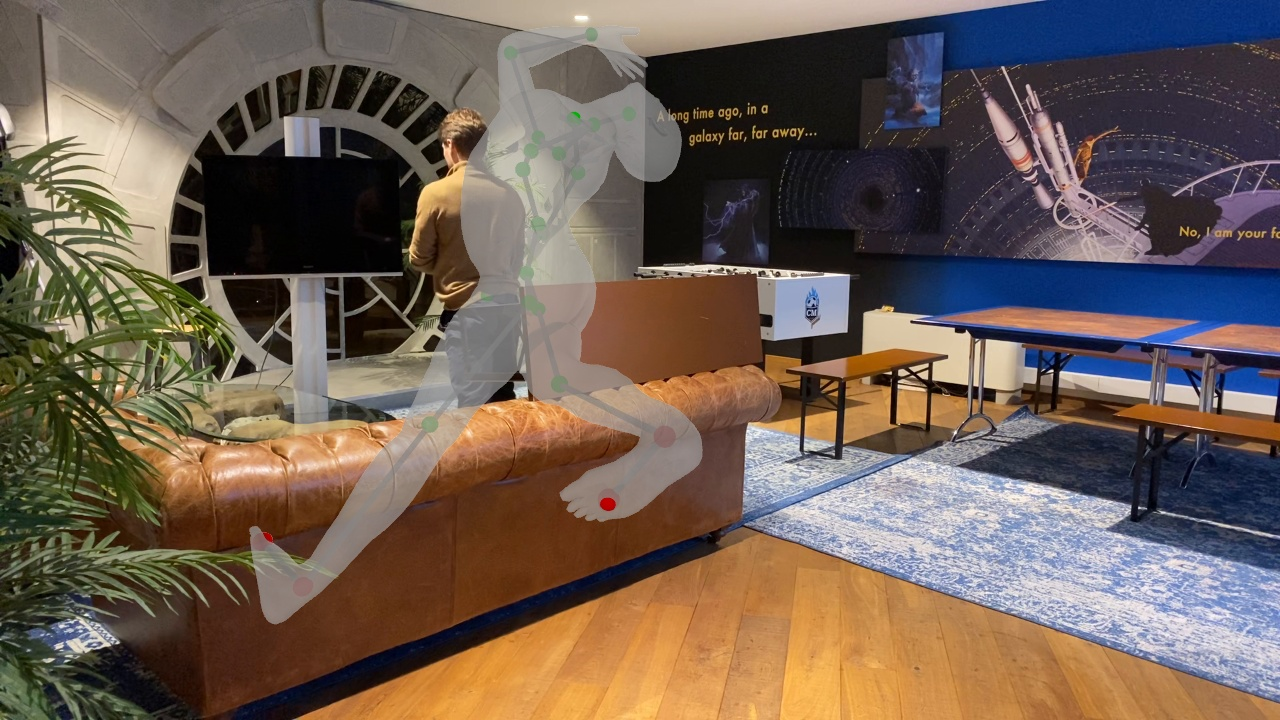
\includegraphics[width=0.3\textwidth]{Figures/humor/improvement/Rollout_stage_2/sitting_clip/rollout/frame_00000150.jpg}}
    \caption{Deviation due to rollout of Stage 2 $z$'s}
    \label{fig:humor_stage_2_rollout_deviation}
\end{figure}


With some preliminary experiments in which we began optimising $x$'s and $z$'s we found that the most successful approach to blending the decoded and optimised $x$'s was to have an L1 loss on the distance between them. We saw that when simply copying over, the propagation of small errors forward was too strong (as desribed in \figref{fig:humor_stage_2_rollout_deviation}) and the system failed to recover as the long range gradients present in the HuMoR TestOps method weren't present, and we found when blending rather than completely copying over that the weighting of the blending was another parameter that was difficult to choose, hence having a loss was the path of least resistence.

Next we experimented with jointly optimising $x$ and $z$ with a larger variety of losses. It was noted that the sitting down motion was not acheived consistenly. However as previously mentioned, the initial $z$'s encode a sitting motion, thus we conject that the $x$'s and $z$'s were fighting and this sitting motion was lost, that is to say the $z$'s move to match the $x$'s motion in which the skeleton simply clips into the floor without bending legs, thus the $z$'s begin encoding less leg bending. To avoid this issue in future experiments, the $z$'s were detached from the consistency loss making the optimised $x$'s match the decoded $x$'s.

This led us on to some experiments in which we either optimise $z$ whilst fixing $x$, or vice versa. With the $z$'s fixed at the stage 2 results, we managed to acheive a sensible sitting motion for a clip containing occluded sitting, but when we applied the same optimiser settings to a longer clip the results were no longer satisfactory. We also noted that when it did work, it required a large number of iterations, in the 1000s, which took 10mins or more, thus the speedup was not as evident as hoped (though our method would continue scaling better). In the inverse case, fixing $x$ to the final HuMoR optimised states and optimising $z$, we noted that we consistently converge in the direction of the final HuMoR $z$'s, which indicates that we are optimising in the right direction, with the best results acheived at a rollout of 5 decoding steps.

All these experiments were performed with varying numbers of decoding steps, 1, 2, 5, and 10. We found that the effect of more stable results but slower compute times with longer rollouts did manifest as intuition would suggest. 

These experiments suggest that the next direction to pursue would be an optimisation scheme in which we flip flop optimising $z$ then $x$. However considering our difficulty in achieving consistent results for the optimisation of the $x$'s with fixed $z$'s, our feeling that this might not be the optimal solution to the problem, my desire to try a new direction, and the time constraints, we deemed it time to move on and try a new method.

\subsection{Conclusion}

We found that jointly optimising the $x$'s and $z$'s did not prove an easy task to solve, which may indicate that
\begin{itemize}
    \item it is a particularly difficult problem, and therefore that the optimiser struggles to satisfy the constraints and find a good minimum for both $x$ and $z$ at the same time
    \item the coupling of the $x$'s and $z$'s in the HuMoR decoder is an important issue. We found it to be at least a minor issue as it was necessary to decouple the $z$'s from the consistency loss (matching the optimised $x$s to the decoded $x'$'s) to avoid the $z$'s being modified in such a way as to fit the unoptimised $x$'s at the beginning of the optimisation
    \item the optimiser is badly balanced
\end{itemize}
This at the very least suggests that a new decoder that does not couple $x$'s and $z$'s would be useful and worth investigating if a similar method is pursued.

In the investigations we found it possible to acheive sensible results on a given clip (for example fixing the unoptimised initial $z$'s, we can a plausible sitting motion in a small video of sitting in occlusion) but that the same settings for the optimiser failed to acheive a good result on an alternative clip. This may indicate that 
\begin{itemize}
    \item again, this is a difficult problem that the optimiser will struggle to solve
    \item the optimiser is badly balanced
\end{itemize} as before.

While many of the issues encountered may simply be due to a badly balanced optimiser, considerable effort was made to mitigate this potential issue, and therefore it is our impression that this problem is at the very least a difficult one. We have improved our intuition, fixed several issues, and understood more about the problem and our goals. We therefore can make a more informed decision with respect to which direction to pursue next. \\
We found that taking a system that was designed with autogregression in mind, and trying to parrallelise it, proved more difficult than expected. The experiments lead us to beleive that jointly optimising a sequence of poses and latent variables obtained through a single frame decoder may be a more difficult formulation of the problem than others. We therefore conclude that a method in which we model longer motion sequences may be more fruitful.

\TODO{Double check through Notes/Current\_experiments.md to see if there's anything else we can learn from the experiments}
\chapter{Conclusion and Outlook}

\TODO{Chpt 1}

% ---- END MAIN PART ----


\appendix
\clearpage
\renewcommand*{\chapterpagestyle}{myappendixpagestyle}

\chapter{Information For The Few}

Nein, meine Texte les ich nicht, so nicht, st?hnte Oxmox. Er war mit Franklin, Rockwell und dem halbtaxgrauen Panther Weidemann in Memphis (Heartbreak Hotel) zugange. Sie warteten auf die fette Gill, um bei der Bank of Helvetica die Kapit?lchen in Kapital umzuwandeln. Oxmox liess nicht locker. Ich fleh euch an, rettet meine Copy, gebt meinem Body nochn Durchschuss! Kein Problem, erbarmte sich Old Face Baskerville, streichelte seinen Hund, zog seine einspaltige Poppl, legte an und traf! (Zeidank nichts Ernstes --- nurn bisschen Fraktur.) Oxmox: Danke, ist jetzt mit Abstand besser. Derweil jumpte der Fox leise over the Buhl, die sich mal wieder immerdar wie jedes Jahr gesellte. Diesmal war Guaredisch ihr Erw?hlter, weil seine Laufweite einem vollgetankten Bodoni entsprach und seine ungez?gelte Unterl?nge ihre Serifen so serafisch streifte, dass sie trotz Techtelmechtelei die magere Futura, jene zuverl?ssige und gern eingesetzte Langstreckenl?uferin, rechtsb?ndig ?berholen konnten.

\section{Foo Bar Baz}

Nein, meine Texte les ich nicht, so nicht, st?hnte Oxmox. Er war mit Franklin, Rockwell und dem halbtaxgrauen Panther Weidemann in Memphis (Heartbreak Hotel) zugange. Sie warteten auf die fette Gill, um bei der Bank of Helvetica die Kapit?lchen in Kapital umzuwandeln. Oxmox liess nicht locker. Ich fleh euch an, rettet meine Copy, gebt meinem Body nochn Durchschuss! Kein Problem, erbarmte sich Old Face Baskerville, streichelte seinen Hund, zog seine einspaltige Poppl, legte an und traf! (Zeidank nichts Ernstes --- nurn bisschen Fraktur.) Oxmox: Danke, ist jetzt mit Abstand besser. Derweil jumpte der Fox leise over the Buhl, die sich mal wieder immerdar wie jedes Jahr gesellte. Diesmal war Guaredisch ihr Erw?hlter, weil seine Laufweite einem vollgetankten Bodoni entsprach und seine ungez?gelte Unterl?nge ihre Serifen so serafisch streifte, dass sie trotz Techtelmechtelei die magere Futura, jene zuverl?ssige und gern eingesetzte Langstreckenl?uferin, rechtsb?ndig ?berholen konnten.

\section{Barontes}

Nein, meine Texte les ich nicht, so nicht, st?hnte Oxmox. Er war mit Franklin, Rockwell und dem halbtaxgrauen Panther Weidemann in Memphis (Heartbreak Hotel) zugange. Sie warteten auf die fette Gill, um bei der Bank of Helvetica die Kapit?lchen in Kapital umzuwandeln. Oxmox liess nicht locker. Ich fleh euch an, rettet meine Copy, gebt meinem Body nochn Durchschuss! Kein Problem, erbarmte sich Old Face Baskerville, streichelte seinen Hund, zog seine einspaltige Poppl, legte an und traf! (Zeidank nichts Ernstes --- nurn bisschen Fraktur.) Oxmox: Danke, ist jetzt mit Abstand besser. Derweil jumpte der Fox leise over the Buhl, die sich mal wieder immerdar wie jedes Jahr gesellte. Diesmal war Guaredisch ihr Erw?hlter, weil seine Laufweite einem vollgetankten Bodoni entsprach und seine ungez?gelte Unterl?nge ihre Serifen so serafisch streifte, dass sie trotz Techtelmechtelei die magere Futura, jene zuverl?ssige und gern eingesetzte Langstreckenl?uferin, rechtsb?ndig ?berholen konnten.


\section{A Long Table with Booktabs}


{\scriptsize
\begin{longtable}{clccccccc}
\caption[wordlist]{A sample list of words.}\\
\toprule
ID & Word & Word Length & WD & ETL & PTL &  WDplus \\
\midrule
\endfirsthead
\caption[]{(Continued)}\\
\toprule
ID & Word & Word Length & WD & ETL & PTL &  WDplus \\
\midrule
\endhead
\midrule
\multicolumn{9}{c}{continued on next page}\\
\bottomrule
\endfoot
%\bottomrule
\endlastfoot
\hline
1 & Eis & 3 & 4 & 0.42 & 1.83 & 0.19 \\ \hline
2 & Mai & 3 & 5 & 0.49 & 1.92 & 0.19 \\ \hline
3 & Art & 3 & 5 & 0.27 & 1.67 & 0.14 \\ \hline
4 & Uhr & 3 & 5 & 0.57 & 1.87 & 0.36 \\ \hline
5 & Rat & 3 & 5 & 0.36 & 1.71 & 0.14 \\ \hline
6 & weit & 4 & 6 & 0.21 & 1.65 & 0.25 \\ \hline
7 & eins & 4 & 6 & 0.38 & 1.79 & 0.26 \\ \hline
8 & Wort & 4 & 6 & 0.30 & 1.62 & 0.20 \\ \hline
9 & Wolf & 4 & 6 & 0.18 & 1.54 & 0.19 \\ \hline
10 & Wald & 4 & 6 & 0.31 & 1.63 & 0.19 \\ \hline
11 & Amt & 3 & 6 & 0.30 & 1.67 & 0.14 \\ \hline
12 & Wahl & 4 & 7 & 0.36 & 1.77 & 0.42 \\ \hline
13 & Volk & 4 & 7 & 0.45 & 1.81 & 0.20 \\ \hline
14 & Ziel & 4 & 7 & 0.48 & 1.78 & 0.42 \\ \hline
15 & vier & 4 & 7 & 0.38 & 1.81 & 0.42 \\ \hline
16 & Kreis & 5 & 7 & 0.26 & 1.62 & 0.33 \\ \hline
17 & Preis & 5 & 7 & 0.28 & 1.51 & 0.33 \\ \hline
18 & Re-de & 4 & 7 & 0.22 & 1.56 & 0.33 \\ \hline
19 & Saal & 4 & 7 & 0.75 & 2.10 & 0.43 \\ \hline
20 & voll & 4 & 7 & 0.48 & 1.82 & 0.24 \\ \hline
21 & weiss & 5 & 7 & 0.21 & 1.59 & 0.36 \\ \hline
22 & ?r-ger & 5 & 7 & 1.16 & 2.69 & 0.59 \\ \hline
23 & bald & 4 & 7 & 0.18 & 1.56 & 0.19 \\ \hline
24 & hier & 4 & 7 & 0.40 & 1.70 & 0.43 \\ \hline
25 & neun & 4 & 7 & 0.17 & 1.52 & 0.26 \\ \hline
26 & sehr & 4 & 7 & 0.36 & 1.85 & 0.43 \\ \hline
27 & Jahr & 4 & 7 & 0.50 & 1.82 & 0.43 \\ \hline
28 & Gold & 4 & 7 & 0.04 & 1.35 & 0.20 \\ \hline
29 & T?-ter & 5 & 8 & 0.15 & 1.39 & 0.59 \\ \hline
30 & Tei-le & 5 & 8 & 0.30 & 1.71 & 0.46 \\ \hline
31 & Na-tur & 5 & 8 & 0.18 & 1.59 & 0.41 \\ \hline
32 & Feu-er & 5 & 8 & 0.30 & 1.71 & 0.45 \\ \hline
33 & Rol-le & 5 & 8 & 0.15 & 1.46 & 0.45 \\ \hline
34 & Rock & 4 & 8 & 0.29 & 1.68 & 0.25 \\ \hline
35 & Spass & 5 & 8 & 0.28 & 1.64 & 0.32 \\ \hline
36 & G?s-te & 5 & 8 & 0.49 & 1.75 & 0.66 \\ \hline
37 & En-de & 4 & 8 & 0.36 & 1.72 & 0.33 \\ \hline
38 & Kunst & 5 & 8 & 0.26 & 1.59 & 0.35 \\ \hline
39 & Li-nie & 5 & 8 & 0.45 & 1.88 & 0.63 \\ \hline
40 & B?u-me & 5 & 8 & 0.48 & 1.92 & 0.45 \\ \hline
41 & B?h-ne & 5 & 9 & 0.94 & 2.48 & 0.62 \\ \hline
42 & Bahn & 4 & 9 & 0.21 & 1.62 & 0.42 \\ \hline
43 & B?r-ger & 6 & 9 & 0.38 & 1.70 & 0.65 \\ \hline
44 & Druck & 5 & 9 & 0.60 & 2.03 & 0.31 \\ \hline
45 & zehn & 4 & 9 & 0.41 & 1.84 & 0.42 \\ \hline
46 & Va-ter & 5 & 9 & 0.36 & 1.78 & 0.40 \\ \hline
47 & Angst & 5 & 9 & 0.29 & 1.56 & 0.35 \\ \hline
48 & lei-der & 6 & 9 & 0.13 & 1.47 & 0.52 \\ \hline
49 & h?u-fig & 6 & 9 & 0.82 & 2.31 & 0.52 \\ \hline
50 & le-ben & 5 & 9 & 0.38 & 1.85 & 0.40 \\ \hline
51 & aus-ser & 6 & 9 & 1.20 & 2.26 & 0.57 \\ \hline
52 & be-vor & 5 & 9 & 1.28 & 2.75 & 0.39 \\ \hline
53 & Kai-ser & 6 & 9 & 0.92 & 2.37 & 0.53 \\ \hline
54 & Markt & 5 & 9 & 0.23 & 1.58 & 0.28 \\ \hline
55 & Os-ten & 5 & 9 & 0.21 & 1.54 & 0.48 \\ \hline
56 & Krieg & 5 & 9 & 0.33 & 1.67 & 0.50 \\ \hline
57 & Mann & 4 & 9 & 0.31 & 1.47 & 0.25 \\ \hline
58 & Hal-le & 5 & 9 & 0.24 & 1.65 & 0.45 \\ \hline
59 & heu-te & 5 & 9 & 0.44 & 1.87 & 0.46 \\ \hline
60 & in-nen & 5 & 10 & 0.36 & 1.80 & 0.45 \\ \hline
61 & Na-men & 5 & 10 & 0.28 & 1.72 & 0.41 \\ \hline
62 & jetzt & 5 & 10 & 0.70 & 2.07 & 0.32 \\ \hline
63 & kei-ner & 6 & 10 & 0.28 & 1.62 & 0.53 \\ \hline
64 & Schu-le & 6 & 10 & 1.02 & 2.12 & 0.48 \\ \hline
65 & Ar-beit & 6 & 10 & 0.34 & 1.70 & 0.52 \\ \hline
66 & An-teil & 6 & 10 & 0.27 & 1.63 & 0.53 \\ \hline
67 & di-rekt & 6 & 10 & 0.67 & 2.04 & 0.47 \\ \hline
68 & vor-her & 6 & 10 & 0.78 & 2.25 & 0.47 \\ \hline
69 & wol-len & 6 & 10 & 0.44 & 1.85 & 0.51 \\ \hline
70 & Kampf & 5 & 10 & 0.70 & 1.96 & 0.27 \\ \hline
71 & ?n-dern & 6 & 10 & 1.18 & 2.62 & 0.65 \\ \hline
72 & lau-fen & 6 & 10 & 0.21 & 1.64 & 0.52 \\ \hline
73 & Eu-ro-pa & 6 & 10 & 0.23 & 1.53 & 0.66 \\ \hline
74 & statt & 5 & 10 & 1.61 & 2.86 & 0.39 \\ \hline
75 & Wes-ten & 6 & 10 & 0.29 & 1.60 & 0.54 \\
\bottomrule
\label{tab:wordlist}
\end{longtable}
}

\clearpage
\renewcommand*{\chapterpagestyle}{empty}

%\nocite{*}
\addcontentsline{toc}{chapter}{Bibliography}
\bibliography{bibliography}

\end{document}
